\documentclass[10pt]{article}
\usepackage{caption}
\usepackage{lipsum}
\usepackage{multicol}
\usepackage{amsmath,amssymb,amsthm}
\usepackage{graphicx}
\usepackage[margin=1in]{geometry}
\usepackage{ragged2e}

\begin{document}

\title{\textbf{Hedging Uniswap Liquidity Positions with GMX Perpetuals and Xtreamly Volatility Forecast}}
\author{
	\small % Reduce font size
	\begin{tabular}{p{7cm}p{7cm}} % Two columns with fixed width
		\textbf{Pawel Masior} & \textbf{Laurens Michiels van Kessenich} \\
		Lotan Group & Xtreamly \\
		\texttt{pawel.masior@lotangroup.com} & \texttt{laurensmvk@gmail.com} \\
		\\ % Add space between authors in the same column
		\textbf{Sogol Malek} & \textbf{Panos Psimatikas} \\
		Xtreamly & Xtreamly \\
		\texttt{sogol.malek1@googlemail.com} & \texttt{ppsimatikas@gmail.com} \\
	\end{tabular}
}
\smallskip
\date{\today}
\maketitle

\begin{abstract}
	This paper explores the use of perpetual futures to hedge Uniswap V4 and V3 concentrated liquidity positions. By integrating short perpetual strategies with Xtreamly’s volatility predictions, liquidity providers can mitigate impermanent loss and potentially profit from price fluctuations. We analyze the effects of volatility forecasts, leverage, funding costs, and liquidation risks on effective risk management. Finally, we apply the hedging strategy to historical LP positions and evaluate its potential to substantially improve the past performance.
\end{abstract}
\medskip
\begin{multicols}{2}


\section{Introduction}
\label{sec:introduction}

Concentrated liquidity provision, as introduced by Uniswap V3 and refined in V4, has revolutionized decentralized trading by allowing liquidity providers to efficiently allocate capital across chosen price ranges. However, despite improvements in capital efficiency, liquidity providers remain highly exposed to downturn losses.

\smallskip
We have built and tested a hedging strategy that utilizes GMX perpetual futures combined with Xtreamly’s proprietary volatility forecasts to systematically reduce downside exposure while preserving the upside potential of Uniswap liquidity positions. Our method dynamically initiates short perpetual exposure to counteract market risk, aiming to protect and deliver net improvement in returns.

\smallskip
We have analyzed 1,385 historical Uniswap V3 positions with over \$190 million in deposited liquidity analyzed during the 4-month back-testing period (2024-12-01 to 2025-03-25), across ETHUSDT, WBTCUSDT, and WBTCUSDC pools. Here are key results:

\begin{itemize}
	\item \textbf{Profit Improvement:} On aggregate level, over \$1.31 million in additional value was recovered across the Uniswap liquidity positions when applying the hedging strategy. When standardized performance of each position the annualized yield (APY) the median improvement with hedging is 30.87\% APY (across all tested positions).
	\item \textbf{Hedging Efficiency:} Each LP was hedged 3–4 times on average, demonstrating dynamic market adaptation while limiting hedging costs of 5\% of position value.
	\item \textbf{Avoided Liquidations:} Less than 1.2\% of all perpetuals were liquidated. This is due to safe leverage levels optimized with Xtreamly AI. Thanks to Xtreamly volatility we managed the risk appetite and avoid early liquidations which can occur with perpetuals trading.
\end{itemize}

\smallskip
This evaluation demonstrates that integrating predictive volatility analytic with derivative hedging is not only viable but materially beneficial for DeFi liquidity providers. Next, we will expose in detail the hedging mechanism.

\newpage
\section{Hedging Framework}
\label{sec:hedging}

This section outlines key components of the strategy: the Uniswap LP position, the GMX perpetual futures contract, and Xtreamly’s volatility forecasting component.

\subsection{Uniswap LP Position}
\label{sec:uniswaplp}

\subsubsection{Overview}
Consider a LP position in the Uniswap pool within \textit{concentrated liquidity} (CL) as the liquidity is bounded within a range of lower and upper price. To keep real world intuition, let's consider $token_0$ as the volatile asset and $token_1$ as the stable asset value.

\subsubsection{Uniswap V4 Hook Architecture}
Uniswap V4 introduces a modular and extensible architecture through its "hook" smart contracts, enabling to customize pool behavior triggers with own logic. The hook approach creates a bridge between on-chain liquidity provision and off-chain or cross-protocol hedging with real-time triggers:

\begin{itemize}
    \item \textbf{Before Swap}: This activates prior to a swap to send a signal to an external system for hedging action.	
	\item \textbf{After Swap}: This activates after a swap is executed to flag the LP hedging status.
\end{itemize}

\subsubsection{LP Impermanent Loss}

\textit{Impermanent loss} (IL) occurs when the prices of tokens in a liquidity pool diverge from their initial values, reducing the LP position’s value in USD. 

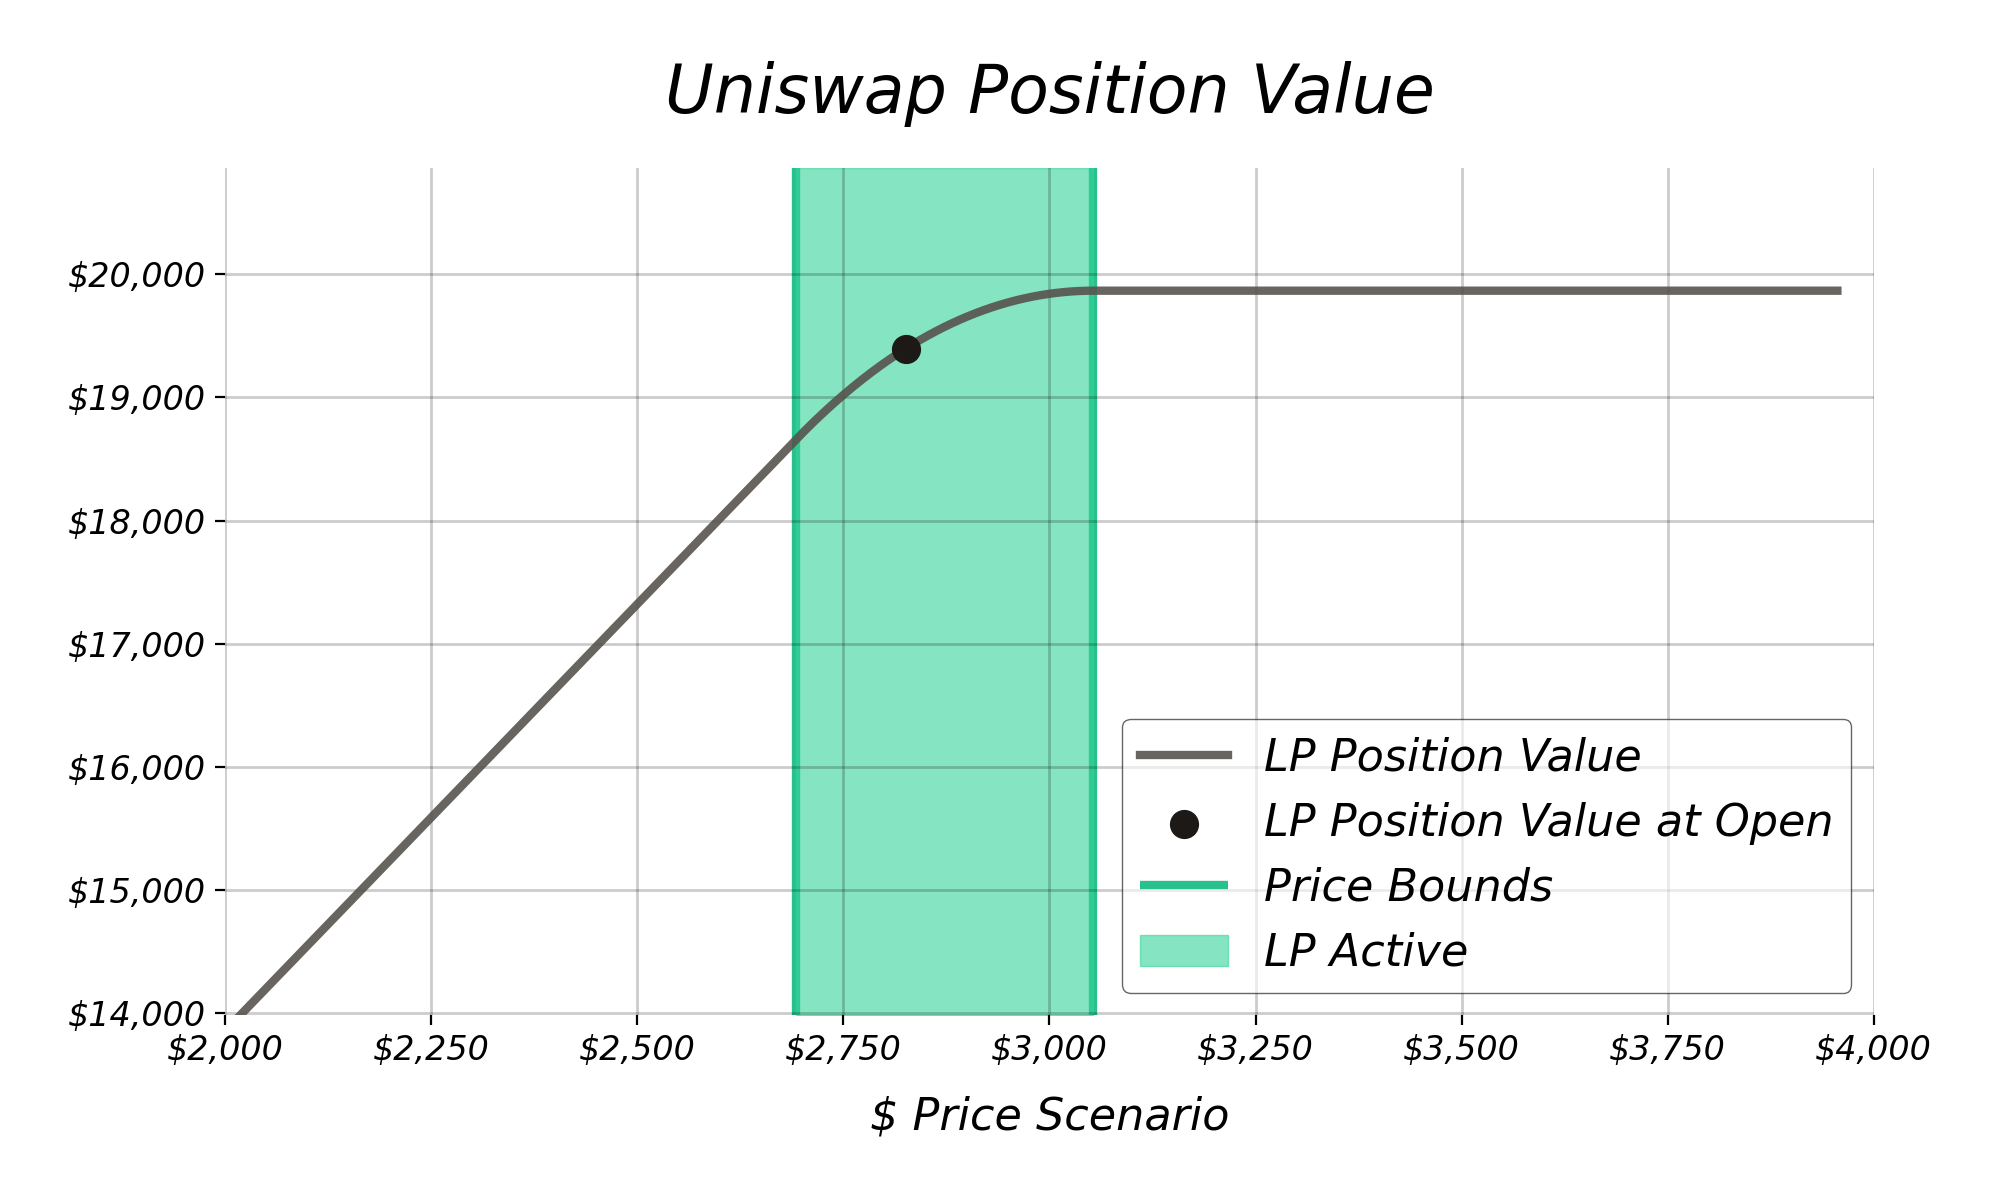
\includegraphics[width=\columnwidth]{img/UniswapPosition.png}
\captionof{figure}{LP Position Value vs. Price Scenarios.}
\label{fig:lpvalue}
\medskip

As shown in Figure~\ref{fig:lpvalue}, when the $token_0$ price $P$ decreases, the LP position’s value degrades, resulting in impermanent loss. This highlights the need for a hedging strategy to create a market-neutral position, allowing LPs to focus on profitability through collected fees rather than price exposure. 

\subsubsection{LP Collected fees}
Collected fees represent the income of an LP position, serving as a reward for providing liquidity and contributing to the position’s final profitability. As long as the market price $P$ remains within the LP position’s upper and lower bounds, the position is active and accrues fees, which enhance the final LP return. 

\smallskip
For simplicity, we exclude collected fees from this analysis, focusing solely on IL in LP payoff function - Profit and Loss (PnL).

\subsection{GMX Perpetual Futures}
\label{sec:perphedge}

Perpetual futures are derivative contracts that track the spot price of an $token_0$ asset without an expiration date, using a funding rate mechanism to balance costs of long and short positions. 

\subsubsection{Perpetual Components}
The following parameters define a GMX perpetual futures contract in this hedging strategy:
\begin{itemize}
	\item \textbf{Entry Price ($P_0$)}: The $token_0$ price at the time the position is opened, serving as the reference for PnL calculations.
	\item \textbf{Mark Price ($P$)}: The current $token_0$ price, typically derived from an oracle to prevent manipulation, used to calculate unrealized PnL.
	\item \textbf{Collateral ($M$)}: The margin (in $token_1$) posted to open and maintain the position, determining leverage and liquidation risk.
	\item \textbf{Leverage ($L$)}: The ratio of the position’s notional value to the margin, defined as $L = \frac{\alpha P_0}{M}$. Higher leverage amplifies gains and losses, increasing liquidation risk.
	\item \textbf{Notional Size ($\alpha$)}: The size of the perpetual position (in $token_0$ units), representing the hedged $token_0$ exposure: $\alpha = \frac{L \cdot M}{P_0}$.
	\item \textbf{Liquidation Price ($P_{\mathrm{liq}}$)}: The $token_0$ price at which liquidation is triggered and the loss of the entire collateral $M$ occurs. 
	\item \textbf{Funding Rate}: A periodic payment (every hour on GMX) between long and short holders to align the perpetual price with the spot price. Positive rates mean shorts pay longs, while negative rates mean longs pay shorts, impacting profitability.
\end{itemize}

\subsubsection{Perpetual Risks}
Holding Perpetual position introduces risks:
\begin{itemize}
    \item \textbf{Delta Risk}: Changes in $P$ can decrease (or increase) the perpetual position’s market value.
	\item \textbf{Liquidation Risk}: If $P$ exceeds $P_{\mathrm{liq}}$, the position is liquidated, resulting in the loss of collateral.
	\item \textbf{Funding Costs}: Persistent positive funding rates can erode profits over time.
\end{itemize}

\subsubsection{Short Perpetual Strategy}
In a short perpetual position, the return increases as the price drops, proportionally to the notional size $\alpha$. Liquidation occurs when $P$ rises significantly above $P_0$.\footnote{In practice, GMX may use partial liquidations or maintenance margins, but we assume full liquidation at $P_{\mathrm{liq}}$ for simplicity.}

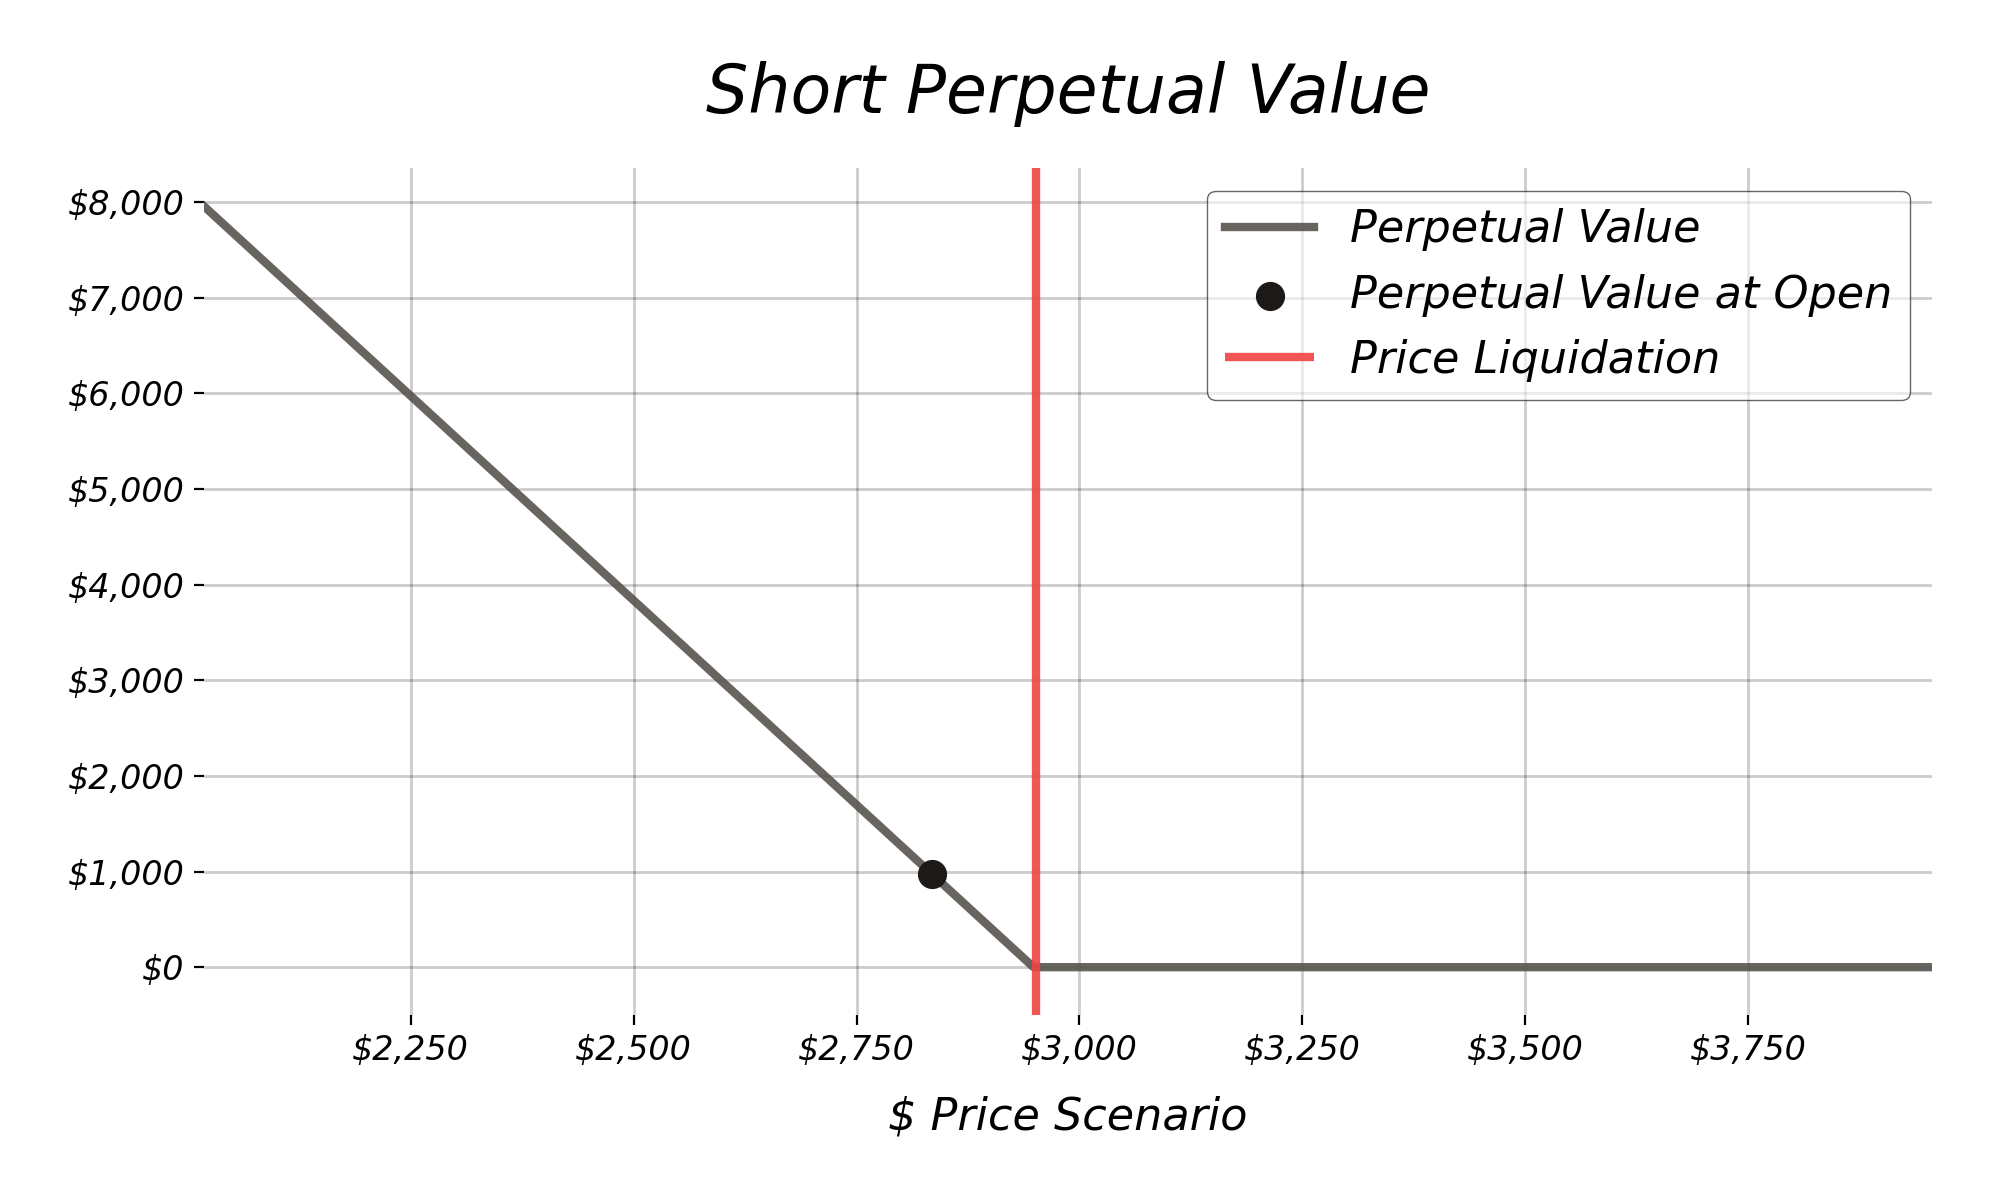
\includegraphics[width=\columnwidth]{img/GMXPosition.png}
\captionof{figure}{Perpetual Value vs. Price Scenarios.}
\label{fig:gmxpayoff}
\smallskip
A short perpetual position can offset impermanent loss (IL) when the $token_0$ price drops, as the perpetual’s gains counterbalance the LP’s losses. For instance, if $P$ decreases, the LP position incurs IL due to pool rebalancing, but the short perpetual gains $\alpha (P_0 - P)$, compensating for the loss. This approach leverages positive delta risk in perpetual to neutralize the delta risk of the LP position.

\subsection{Integrated LP and Perpetual}
\label{sec:fiveway}

This section evaluates the combined Uniswap V4 LP and short GMX perpetual strategy, aiming to dynamically hedge $token_0$ price exposure while optimizing capital efficiency. The goal is to mitigate impermanent loss (IL) while balancing downside protection and potential gains.

\smallskip
As shown in Figure~\ref{fig:perpvalue}, the combined strategy reduces the LP position’s sensitivity to price changes, offering robust protection against IL. Consequently, at a realized price, the LP position’s value remains nearly identical to its value at the entry point, with profits derived primarily from collected fees accumulated during the LP position’s duration.

\smallskip
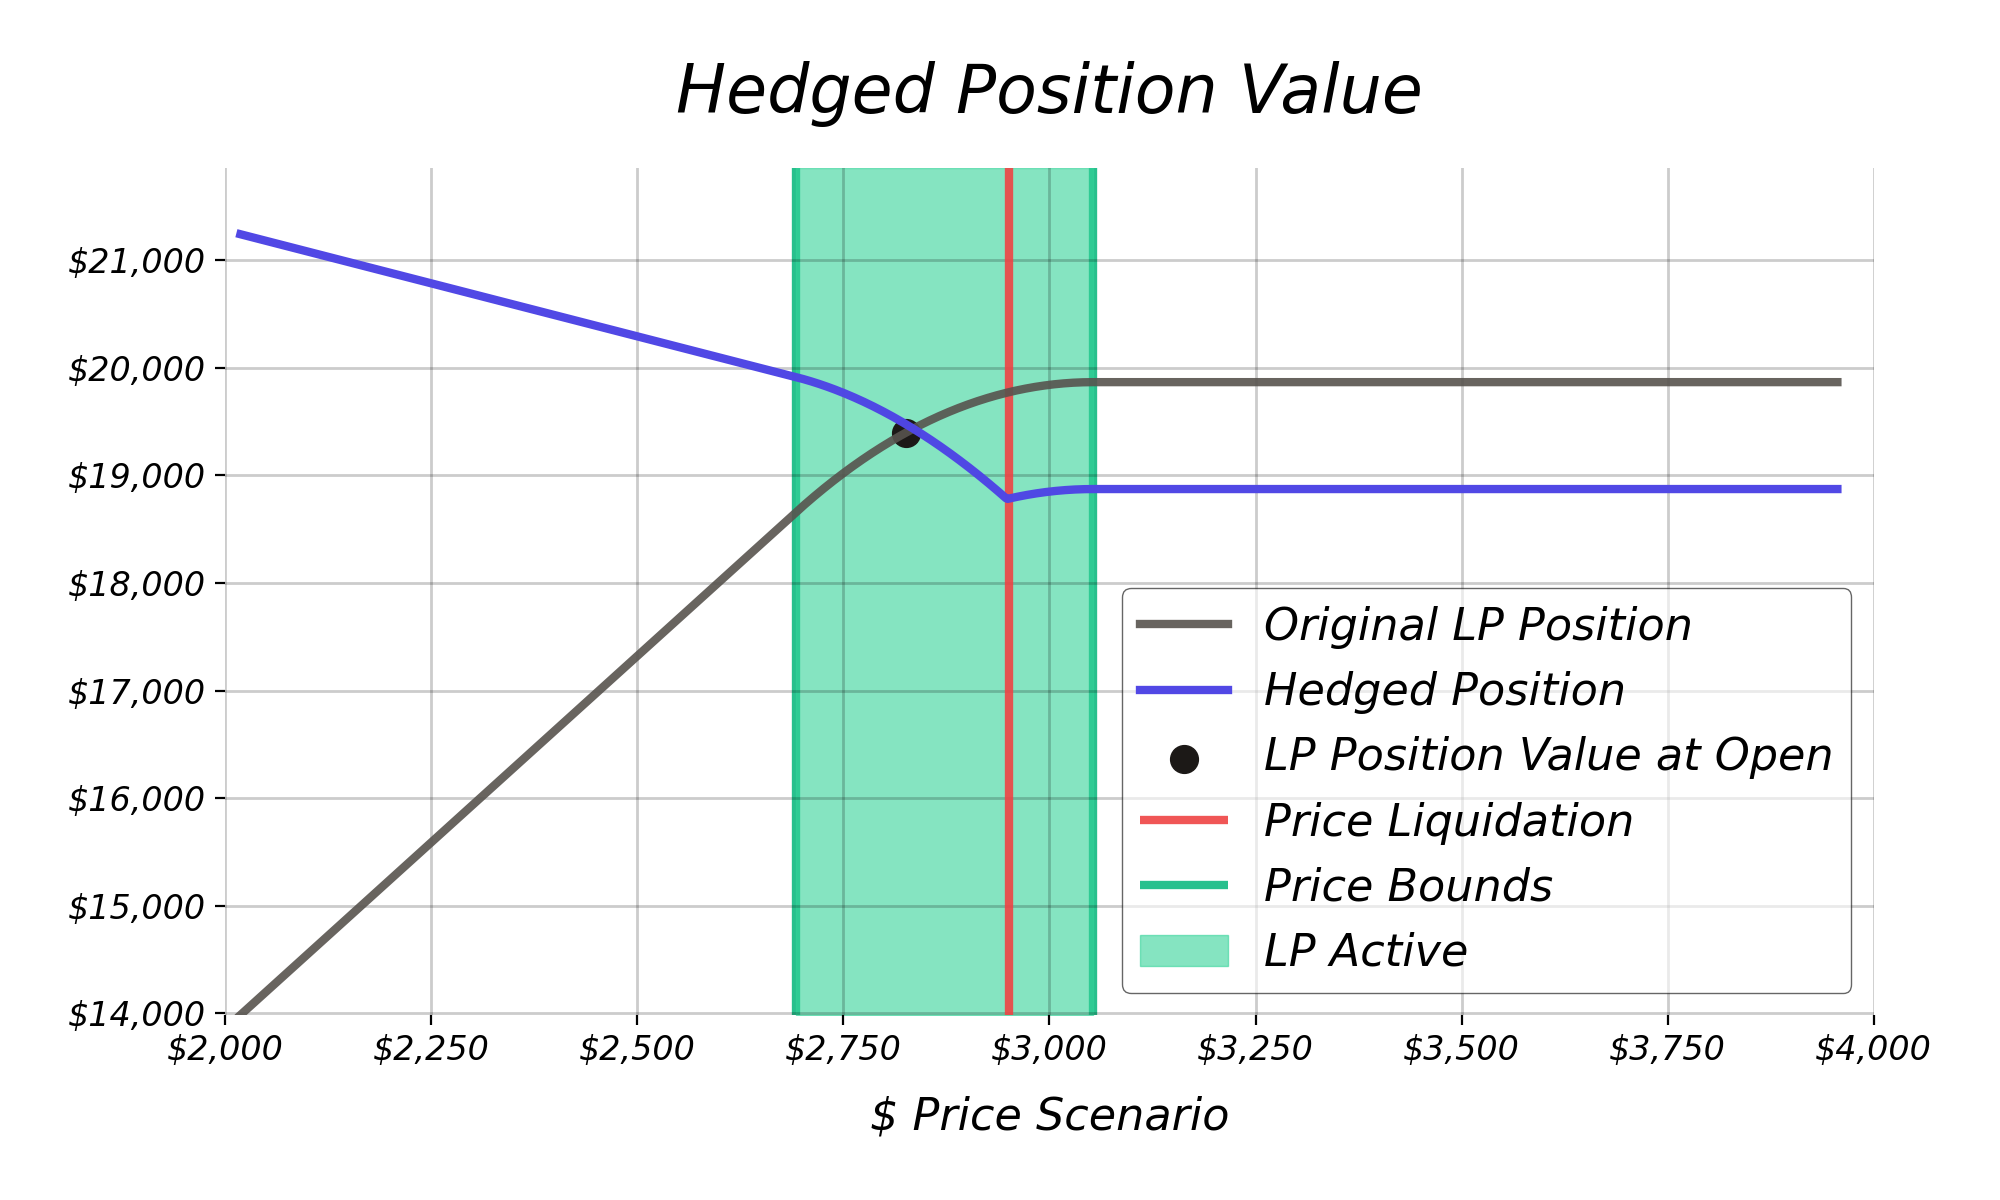
\includegraphics[width=\columnwidth]{img/HedgedPosition.png}
\captionof{figure}{Hedged Position Value vs. Price Scenarios.}
\label{fig:perpvalue}

\subsubsection{Hedging Risks Mitigation}
The strategy’s success depends on careful risk management. The notional size $\alpha$ must balance liquidation risk and capital efficiency. Over-hedging increases exposure to liquidation, while under-hedging fails to mitigate IL. Additionally, an extended holding period may erode profits due to accumulating hedging costs. Here are risk mitigation approaches:
\begin{itemize}
	\item \textbf{Funding Cost}: The cost of holding a perpetual position increases over time. Therefore, a maximum duration must be established to limit accumulative funding costs.
	\item \textbf{Collateral Cost}: The cost of entering a position. This value must be calibrated to avoid consuming too much of the payoff when the price increases, while remaining sufficient to enable effective hedging when the price decreases in final hedged LP position value.
	\item \textbf{Leverage Adjustment}: Higher leverage amplifies returns but increases sensitivity to price swings, funding costs, and liquidation risk. To ensure efficient hedging, leverage must be adjusted to avoid early liquidations triggered by regular market noise, instead of realized price trends.
\end{itemize}

The maximum holding time and fixed collateral costs will be determined through back-testing. However, leverage adjustments can be dynamically defined using Xtreamly’s volatility predictions.

\subsection{Xtreamly Volatility Forecasting}
\label{sec:xtreamly}

Xtreamly’s volatility forecasting enhances the hedging strategy by adjusting leverage in risk management decisions, by reducing the likelihood of premature liquidation. These forecasts enable proactive adjustments to mitigate noise and hedge against adverse price trends.\footnote{We assume that any realized price $P$ after initial price $P_0$ is the combination of trend and noise. This particular approach is widely use in financial engendering like Black-Scholes etc. 
	Hence, with volatility forecasts Xtreamly can take precautions measures to contain the noise and hedge against unfavorable trends.}

\subsubsection{Market States}

Xtreamly categorizes market conditions into three states based on predicted volatility:
\begin{itemize}
	\item \textbf{Low Volatility}: Minimal price movements are expected, allowing for higher leverage.
	\item \textbf{Medium Volatility}: Moderate price movements are anticipated for balanced leverage.
	\item \textbf{High Volatility}: Significant price movements are expected, necessitating lower leverage to avoid early liquidation.
\end{itemize}

\subsubsection{Leverage Adjustment}

Although Xtreamly cannot predict price direction, it uses volatility forecasts to dynamically adjust leverage when opening perpetual positions. During low-volatility periods, higher leverage can enhance profitability by amplifying the hedge’s effectiveness. In high-volatility periods, lower leverage reduces liquidation risk, ensuring the hedge remains active and protects against IL.

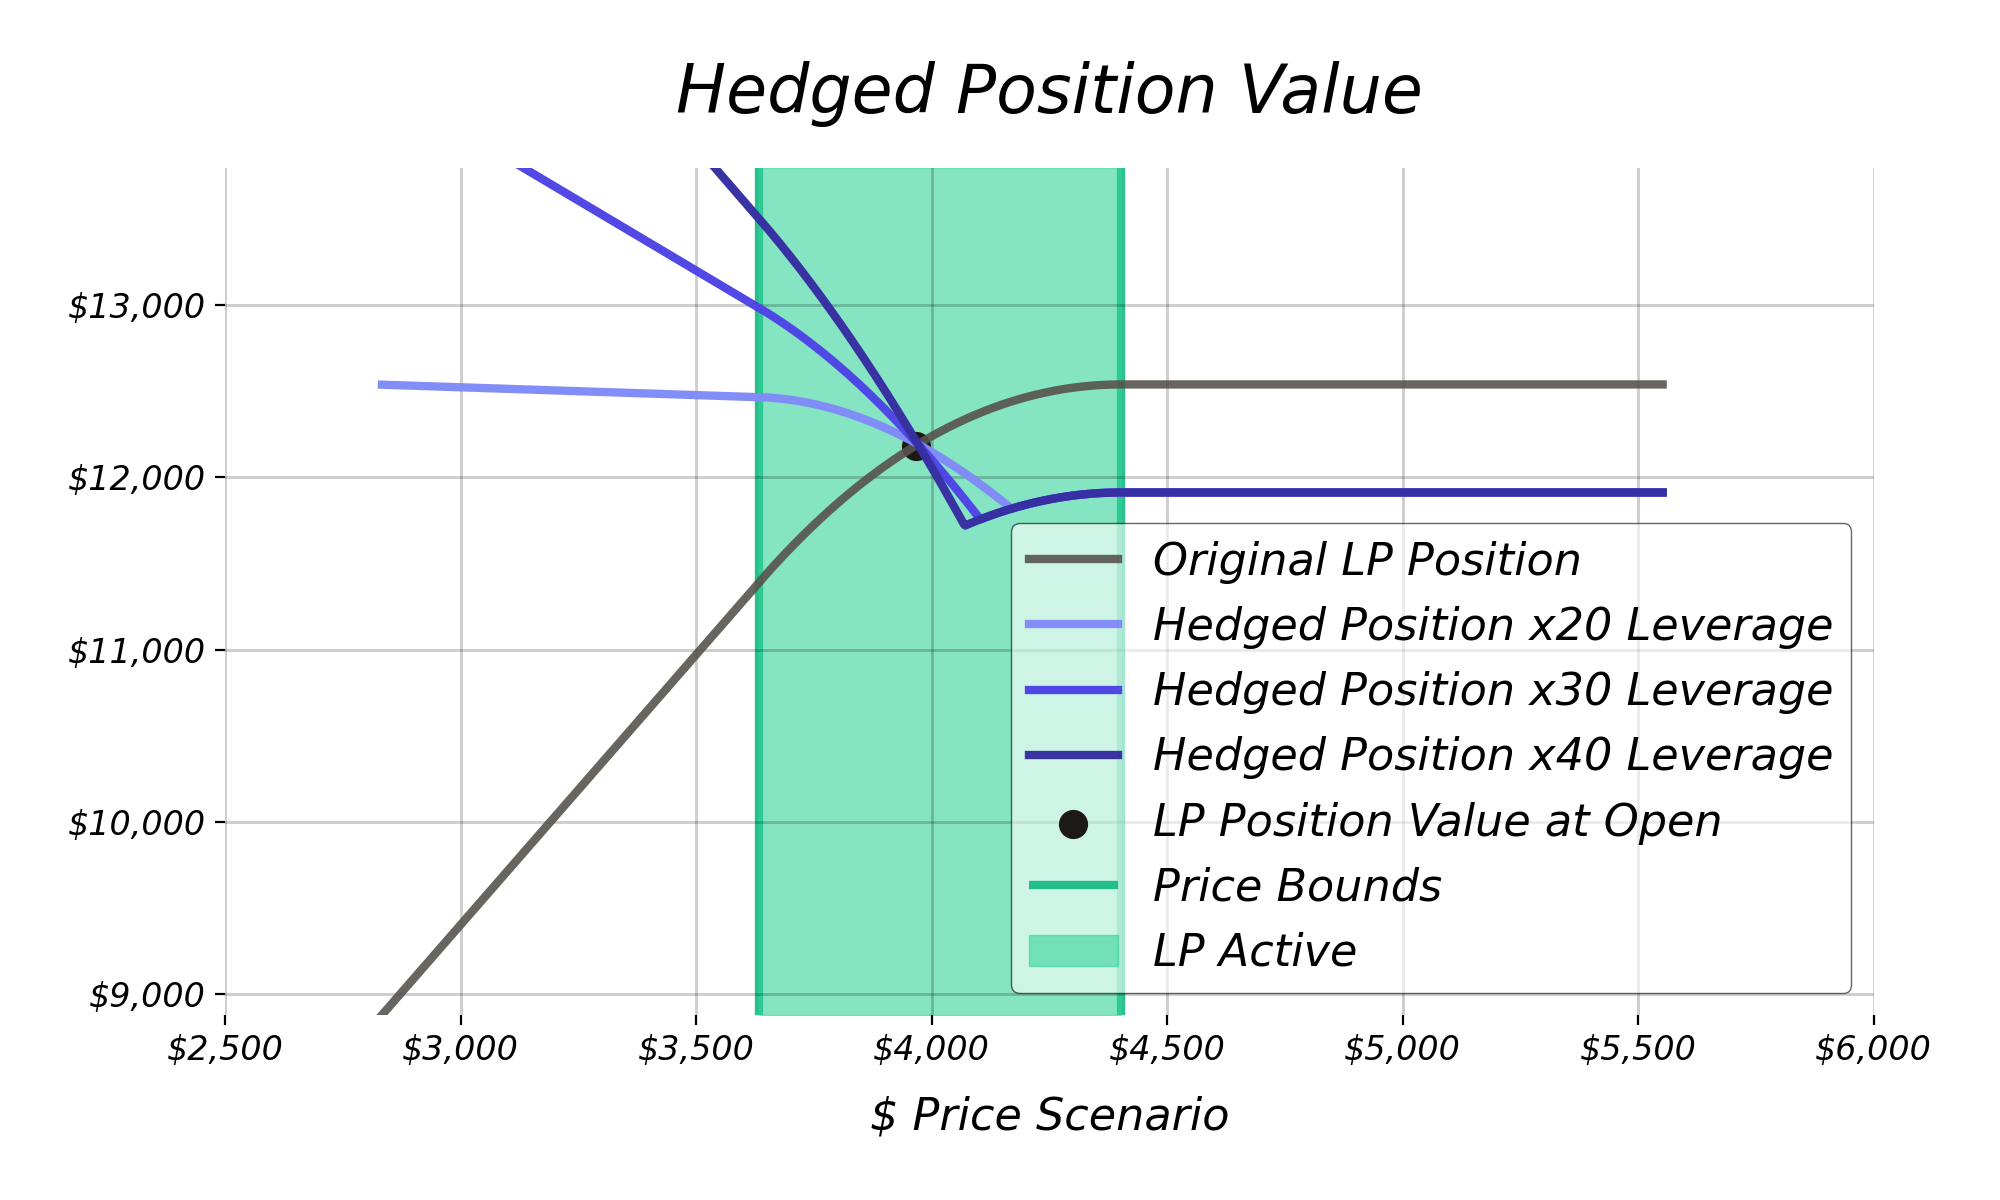
\includegraphics[width=\columnwidth]{img/HedgedPositionLeverage.png}
\captionof{figure}{Hedged Position Value with Various Leverage Levels vs. Price Scenarios.}
\label{fig:hedgedpayoffleverage}
\smallskip

Higher leverage increases positive returns when the price declines. Once liquidations are avoided, the payoff function can also be maximized. Thus, the Xtreamly component is not only critical for determining appropriate leverage but also for maximizing returns whenever the price down trend is realized.

\subsubsection{Collateral Adjustment}
An alternative scenario would involve minimizing collateral costs based on leverage levels. This approach would maintain a delta-neutral strategy but could result in missed hedging opportunities for profits; therefore, it is skipped.

\subsection{Hedging Setup}

\subsubsection{Opening Hedging Perpetual}
The primary motivation for hedging with short perpetuals is to mitigate IL from the very beginning of LP position. This implies that hedging is most effective when initiated at the start of an LP position and can also be applied whenever the price returns to the middle price of $P_L$ and $P_U$:  
$$P_\text{middle} = \frac{1}{2}(P_L+P_U)$$
This approach ties the hedging decision directly to price movements and the current perpetual exposure (when no short perpetual position is active).

\medskip
Specifically, the condition for entering a hedge:
\begin{itemize}
	\item \textbf{Price} $P$ falls within a 1\% interval of $P_\text{middle}$:
	$$P_0 - 1\% \cdot P_0 <= P <= P_\text{middle} + 1\% \cdot P_0$$
	\item \textbf{No Perpetual Opened} This way we allow to have only one short perpetual opened at the same time.
\end{itemize}

\medskip
Once the condition to enter the hedge is satisfied, the perpetual is opened with following actions:
\begin{enumerate}
	\item \textbf{Determine Collateral Amount}. The value $M$ is a proportion of current LP position value.
	\item \textbf{Withdraw Collateral Tokens}: Remove $token_0$ and $token_1$ proportionally to the current LP composition.
	\item \textbf{Swap to Collateral Currency}: Convert the withdrawn tokens into the currency required for the perpetual contract.
	\item \textbf{Set Leverage}: Apply the leverage level determined by the Xtreamly AI engine.
	\item \textbf{Open Short Perpetual}: Submit the order.
\end{enumerate}
These steps ensure that the hedge aligns with the LP position’s exposure and is executed efficiently, minimizing costs and slippage.

\subsubsection{Closing Hedging Perpetual}

The short perpetual hedge will be closed when one of the following conditions is met:
\begin{itemize}
	\item \textbf{Duration} The maximum hold time is reached.
	\item \textbf{Liquidation} The GMX liquidation mechanism has been triggered. In this case, there is no payoff from perpetual. 
	\item \textbf{Closed LP position} Whenever LP position is closed the trigger to close hedging is executed. In this case, the payoff from perpetual is sent directly to LP owner's wallet. 
	\item \textbf{Funding Costs} The funding rate can consume the perpetual value resulting in loss of position. This is highly unlikely as these costs are only a small fraction of the overall position.
\end{itemize}

\medskip

Once the decision to close is made, the position is terminated with following actions:
\begin{enumerate}
	\item \textbf{Close Short Perpetual}: Submit the order.
	\item \textbf{Collect Payoff}: Collect the resulting payoff from the perpetual contract.
	\item \textbf{Swap Payoff to LP Tokens}: Convert the payoff into $token_0$ and $token_1$
	proportionally to the current LP composition. 
	\item \textbf{Deposit Tokens}: Deposit the swapped $token_0$ and $token_1$
	back into the LP position.
\end{enumerate}

\paragraph{Remark}
It is possible, that the signal to close the perpetual coincides with the signal to open it. This could occur only if the realized price at closing simultaneously satisfies the condition for opening a new position. However, this is very unlikely as opening and closing conditions are almost self excluding.

\subsubsection{Optimizing Variables}
The following variables will be optimized for hedging:
\begin{itemize}
	\item \textbf{Maximum Holding Time}: Funding rate payments can erode profits, particularly if positions is held for sufficiently long time.
	\item \textbf{Collateral Allocation}: The collateral determines the hedge’s effectiveness: under-allocating diminishes its impact, while over-allocating is a hedging cost to LP position and affect the PnL. 
	\item \textbf{Leverage Selection}: The formula for effective leverage is determined by Xtreamly market state forecast.
\end{itemize}

\bigskip

\section{Back-testing}

\subsection{Testing Data}
For back-testing, we identified number LP Positions from different pools, that will be used to evaluate the effectiveness of our hedging strategy under different market conditions, comparing LP-only positions against LP positions with perpetual hedging.

\subsubsection{Market Data}
We utilize \textbf{BTC} and \textbf{ETH} minutely prices quoted in \textbf{USD} during 2024-12-01 and 2025-03-25 (the last 4 months) to calculate theoretical performance of GMX perpetuals and interpolate Uniswap positions token amounts and values. 

\smallskip
We have selected most recent period so its most applicable to current market dynamics, It is particularly relevant in light of recent events (ex. presidential elections in United States) that caused significant price swings in BTC and ETH. 

\smallskip
Also, this period resulted in bearish trend for ETH and neutral for BTC making it a perfect playground for testing applicability of hedging. It is necessary for back-testing to cover diverse market scenarios: such as different volatility regimes, price trends to validate the strategy’s robustness and prevent excessive bias.

\subsubsection{Uniswap Data}
To ensure computational simplicity and practical relevance, we select following historical Uniswap V3 positions: 
\begin{itemize}
	\item \textbf{Pools}: We consider ETHUSDT, WBTCUSDT and WBTCUSDC pools in back-testing with fees: 03\% and 0.05\%.
	\item \textbf{Period}: LP positions must have been opened and closed between 2024-12-01 and 2025-03-25.
	\item \textbf{Minimum Duration}:  LP positions with minimum duration 60 minutes, so Just-In-Time (JIT) LP positions are skipped.
	\item \textbf{Concentrated liquidity}: The  spread between $P_L$ and $P_U$ must not exceed 30\% or market price $P$ to ensure the hedging is effective.
	\item \textbf{Basic positions}: Only for simplicity in calculation, we consider LP positions without additional deposits and withdraws during the LP duration.
\end{itemize}
By applying these filters, we ensure realistic hedging conditions where the strategy remains both practical and effective based on sufficient number of pools and LP positions.

\smallskip
\centering
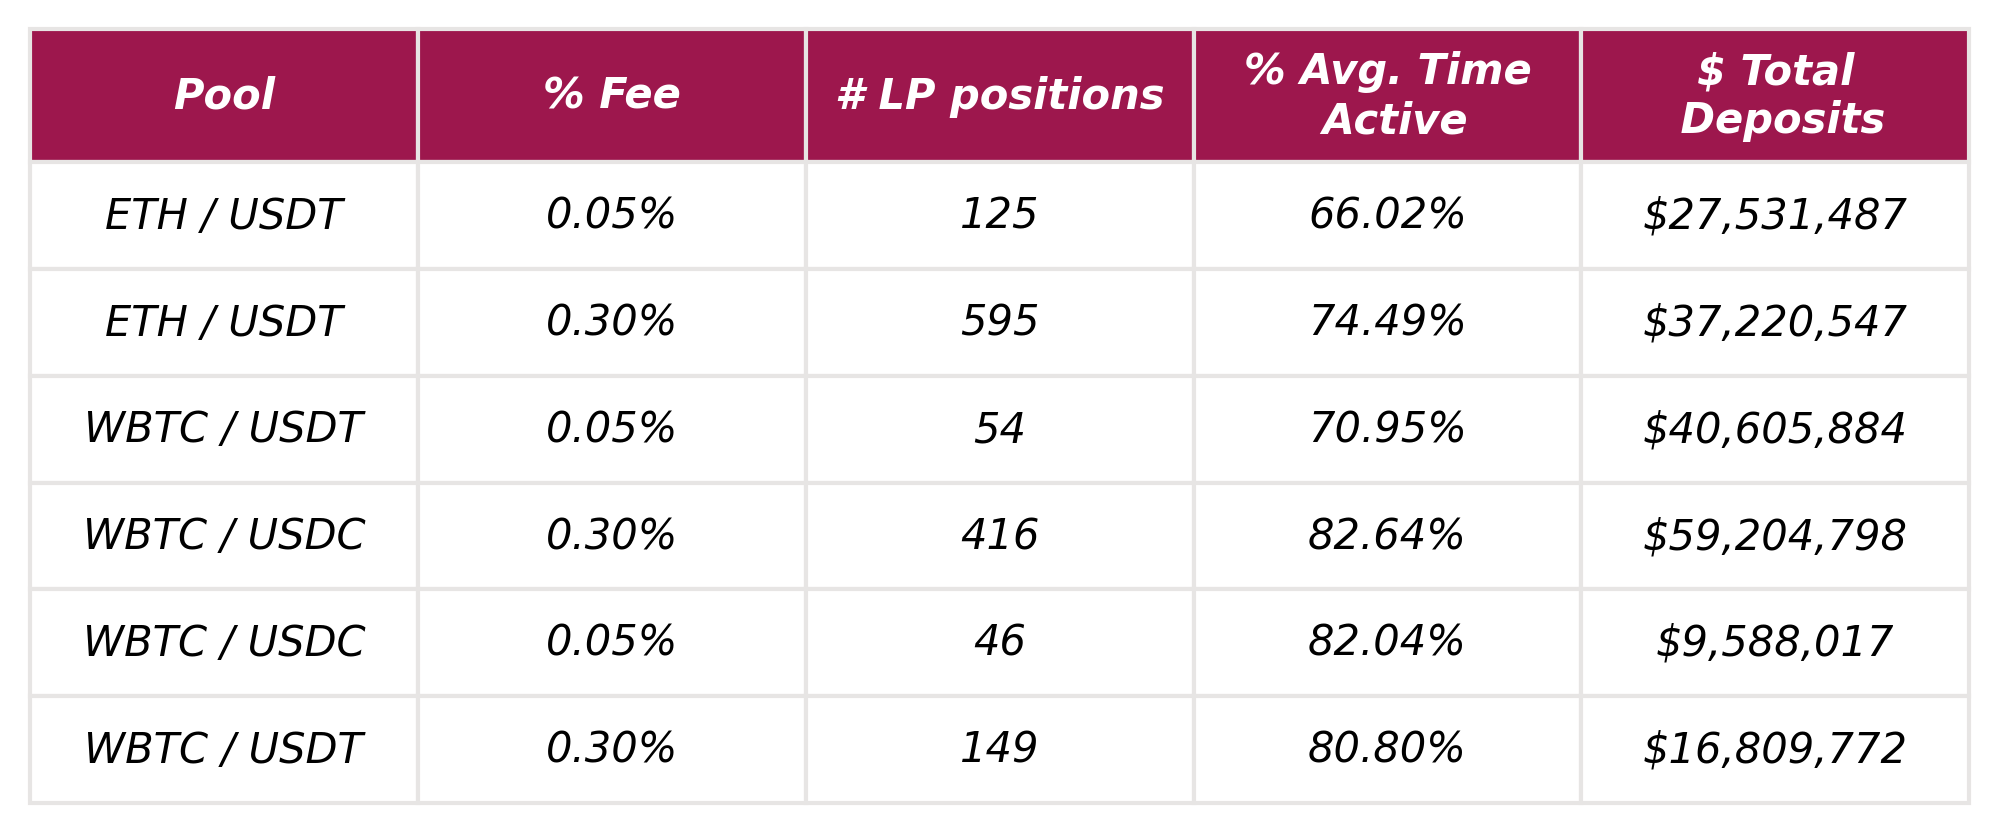
\includegraphics[width=\columnwidth]{img/TblPools}
\captionof{figure}{Historical LP Positions Summary.}
\label{fig:histpools}
\justifying
\smallskip

We have identified around 1,385 candidate LP positions to apply hedging with total deposit value over 190 mln USD. Such testing data is enough to generalize the value of impact of  proposed hedging.

\smallskip
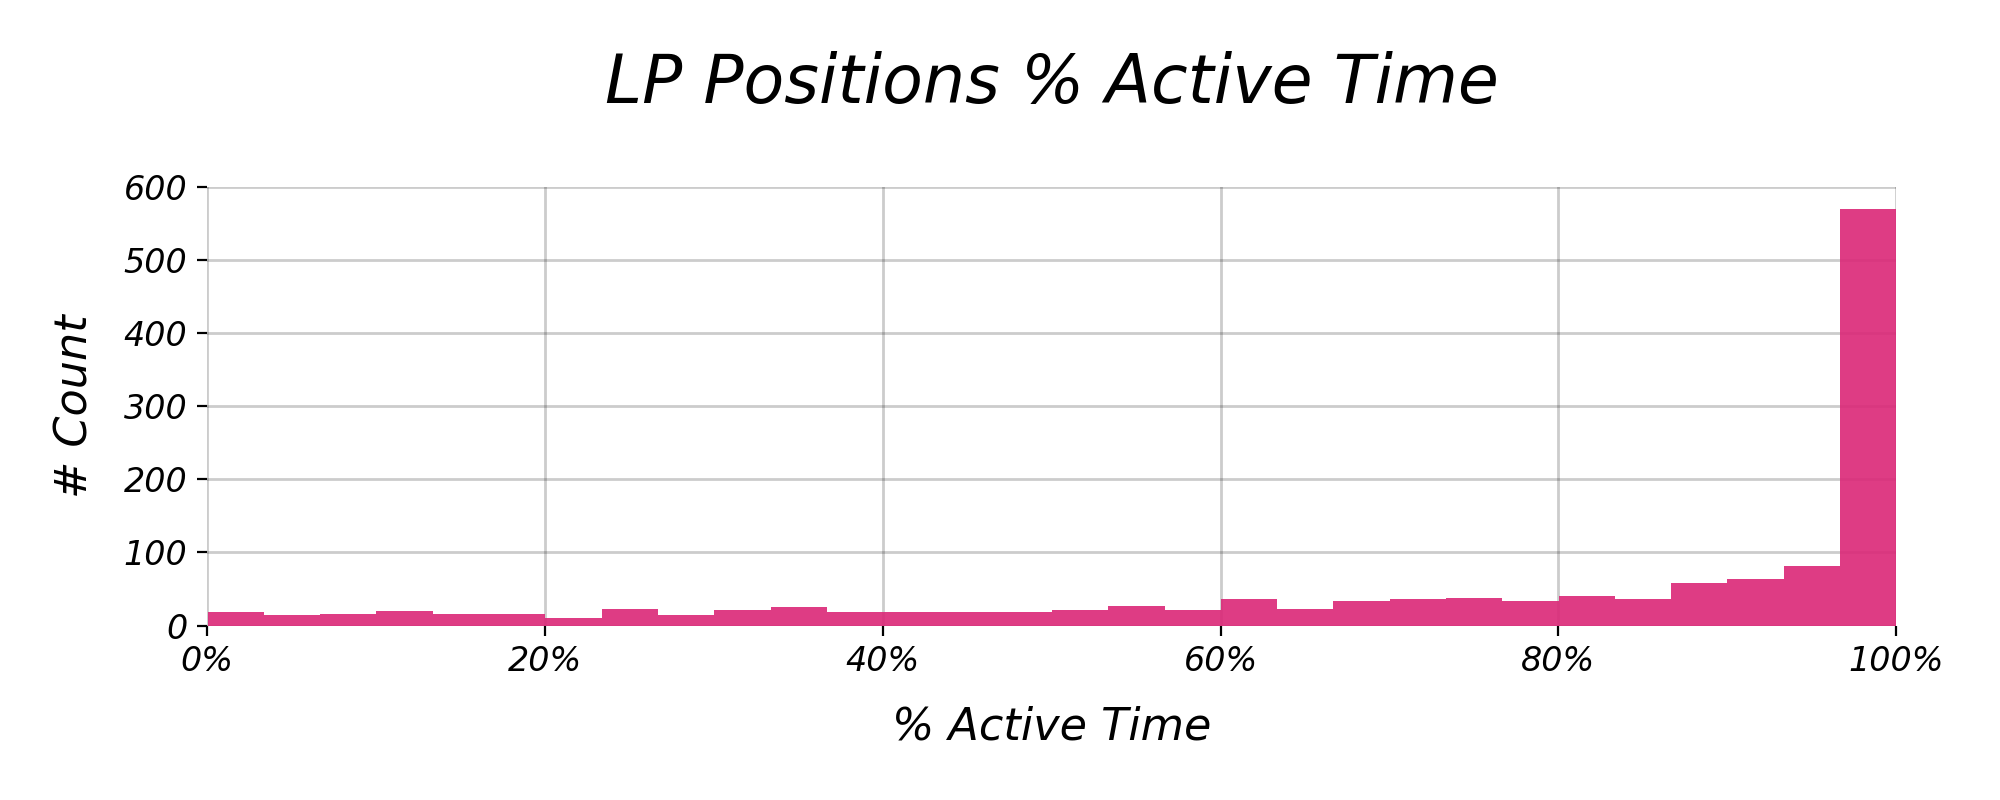
\includegraphics[width=\columnwidth]{img/HistogramActive.png}
\captionof{figure}{Histogram of Share of Time LP Positions were Active.}
\label{fig:HistogramActive}
\smallskip
These positions were on average active for around 70-80\% of time, and most of faced IL.

\subsubsection{Xtreamly Forecasts Data}
We have retrieved historical predictions performed by Xtreamly between 2024-12-01 and 2025-03-25. Xtreamly is already outperforming the industry standards in predicting volatility and can easily apply its data into hedging strategy. 

\smallskip
\centering
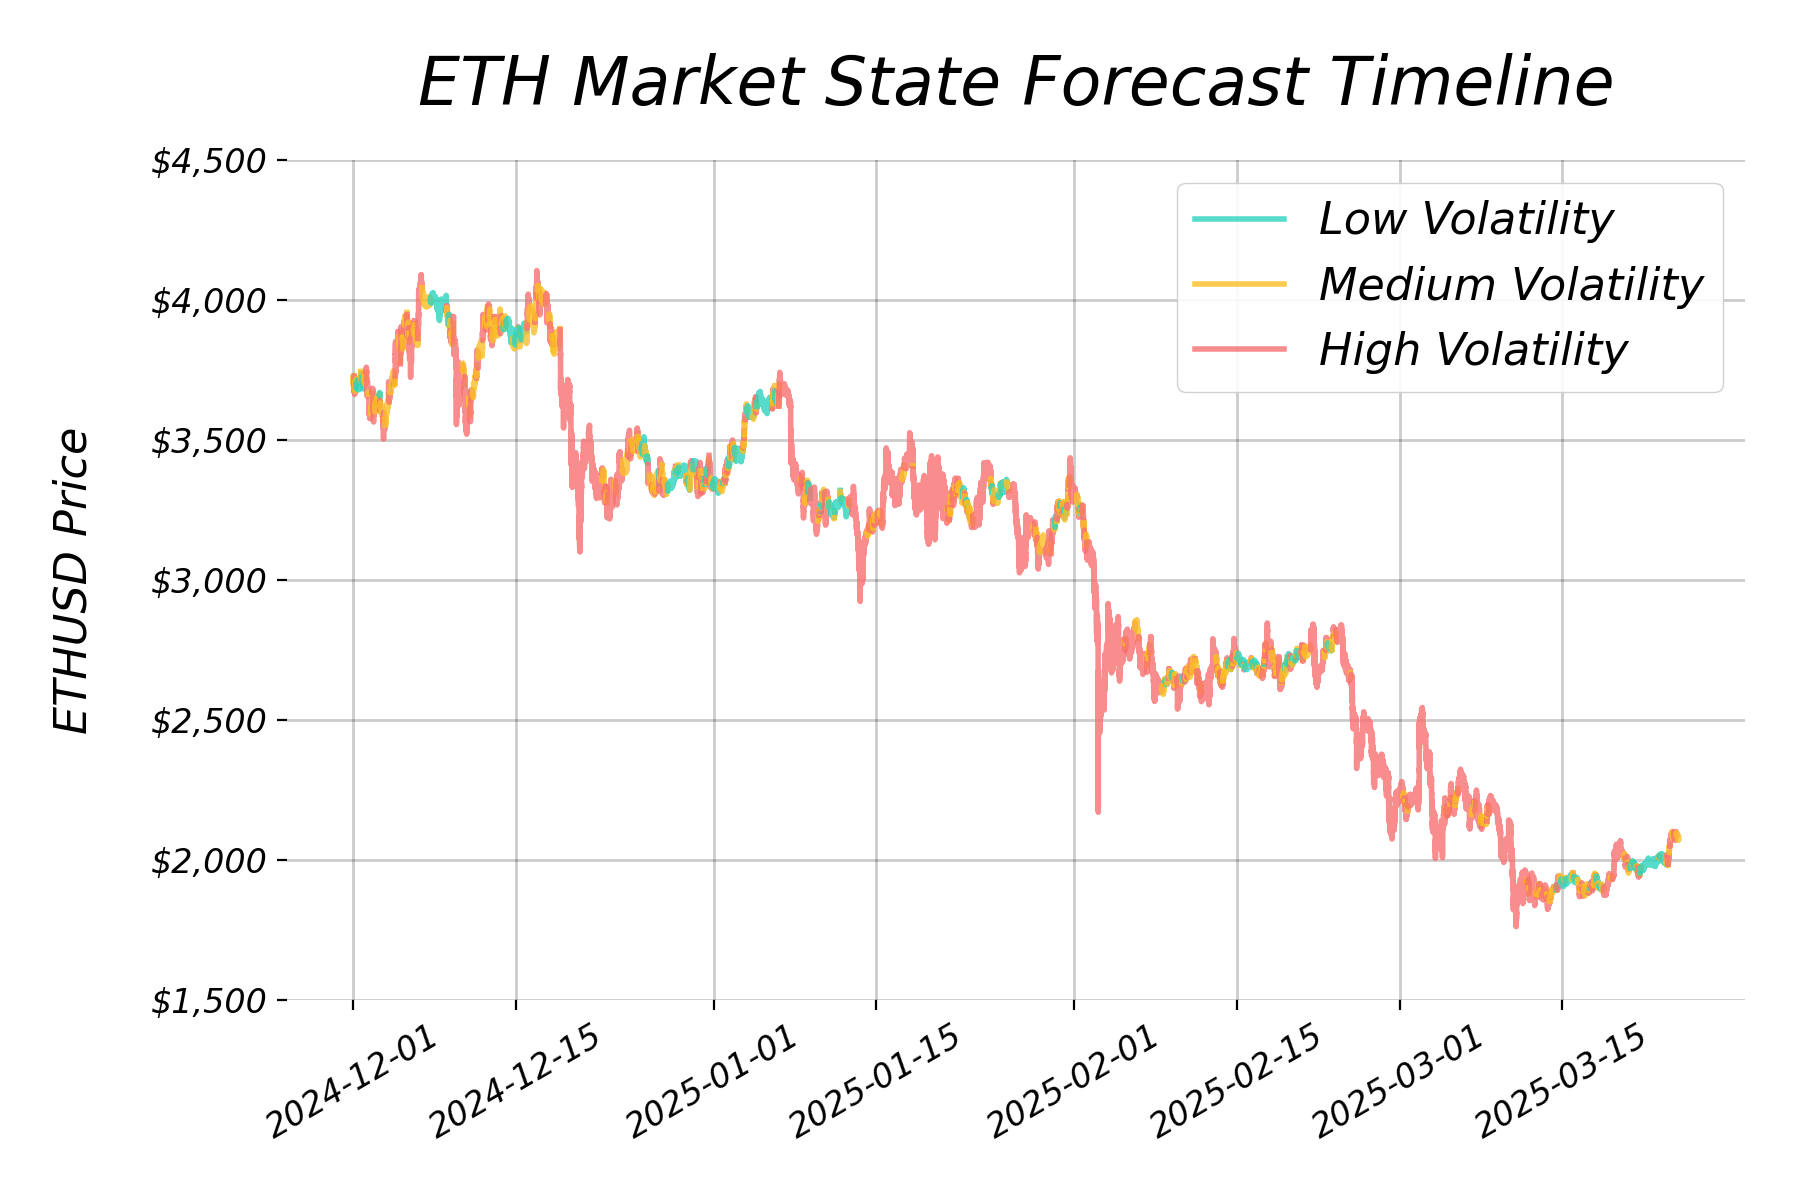
\includegraphics[width=\columnwidth]{img/TimelineForecastMarketStateETH}
\captionof{figure}{ETH Forecasted Market State}
\label{fig:TimelineForecastMarketStateETH}
\justifying

\smallskip
\centering
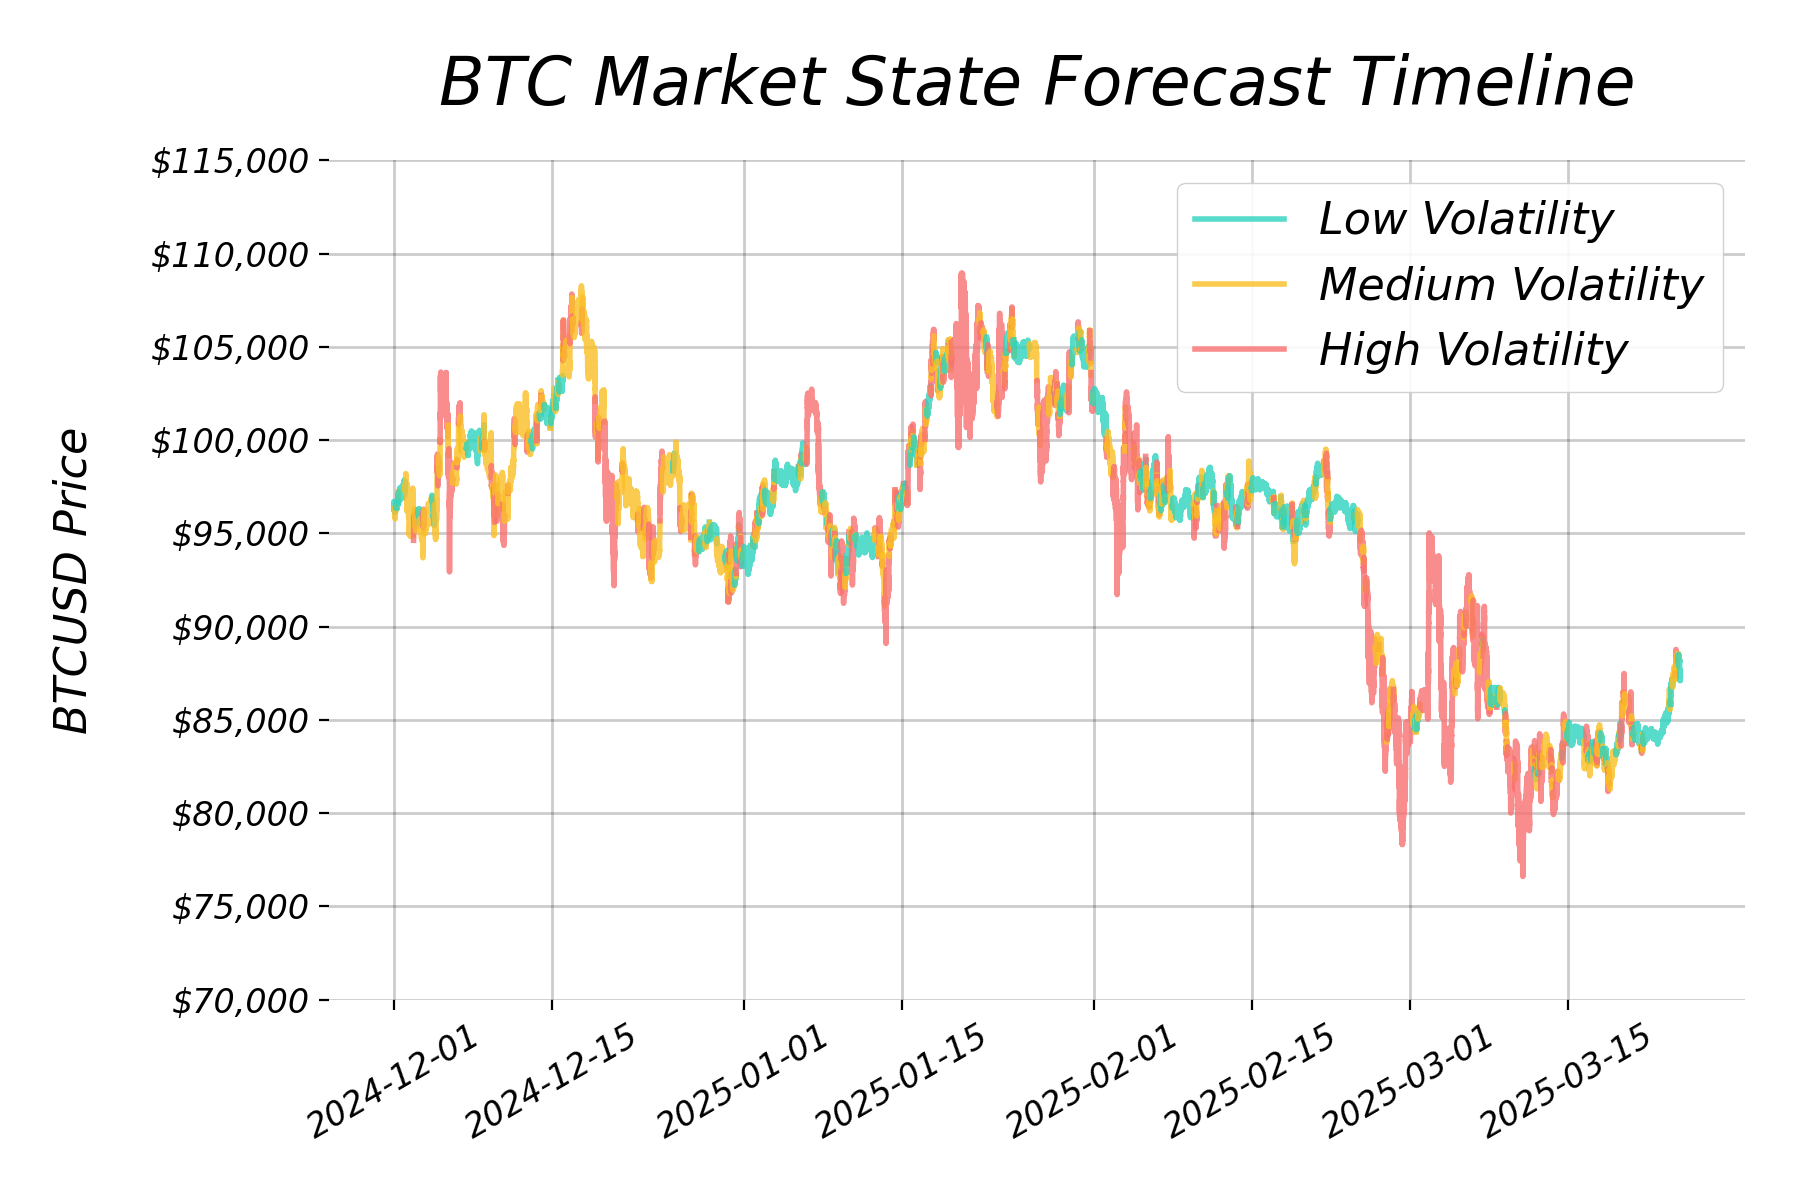
\includegraphics[width=\columnwidth]{img/TimelineForecastMarketStateBTC}
\captionof{figure}{BTC Forecasted Market State}
\label{fig:TimelineForecastMarketStateBTC}
\justifying
\medskip

In the visualized forecasts shown in Figures~\ref{fig:TimelineForecastMarketStateETH} and~\ref{fig:TimelineForecastMarketStateBTC}, we can see empirical good fit of predictions with dominating high volatility periods. While on other periods, especially the low volatility we see not much change in price. This might indicate not only lack of noise but also not material trend. The small movements in price might reduce the positive impact of hedging and so, the higher leverage can be applied.

\subsubsection{Default Fees}

GMX parameters:
\begin{itemize}
	\item \textbf{Entry fee}: 0.1\%
	\item \textbf{Exit fee}: 0.1\%
	\item \textbf{Gas fee}: 0.0\%\footnote{Considered negligible due to GMX's efficient execution model.}
	\item \textbf{Funding rate}: 0.01\%\footnote{For now, assumed constant and charged on an hourly basis. We plan to apply real historic funding rates in the future.}
\end{itemize}

Uniswap V4: for simplicity of calculations and due to efficient of Uniswap V4 architecture, we presume negligible fees on deposit, withdrawn or gas.

\subsection{Results}

\subsubsection{Optimized Variables}
Trough out verifying on various meta parameters, we have identified following numbers:

\begin{itemize}
	\item \textbf{ Maximum Holding Time}: 12 Hours
	\item \textbf{Collateral Allocation}: 5\% of LP Value
	\item \textbf{Leverage Selection}:
	\begin{itemize}
		\item \textbf{Low Volatility}: x30
		\item \textbf{Medium Volatility}: x25
		\item \textbf{High Volatility}: x20			
	\end{itemize}
\end{itemize}

These parameters follow the intuitions: the holding time cannot be too extensive and sufficiently long enough to get materially different new price $P$. The collateral needs to be minimized due to perpetual speculative nature that can consume LP positions value. Lastly, the increasing leverage allows to boost the hedging performance.
\subsubsection{Hedged LP Positions by Pool}

\centering
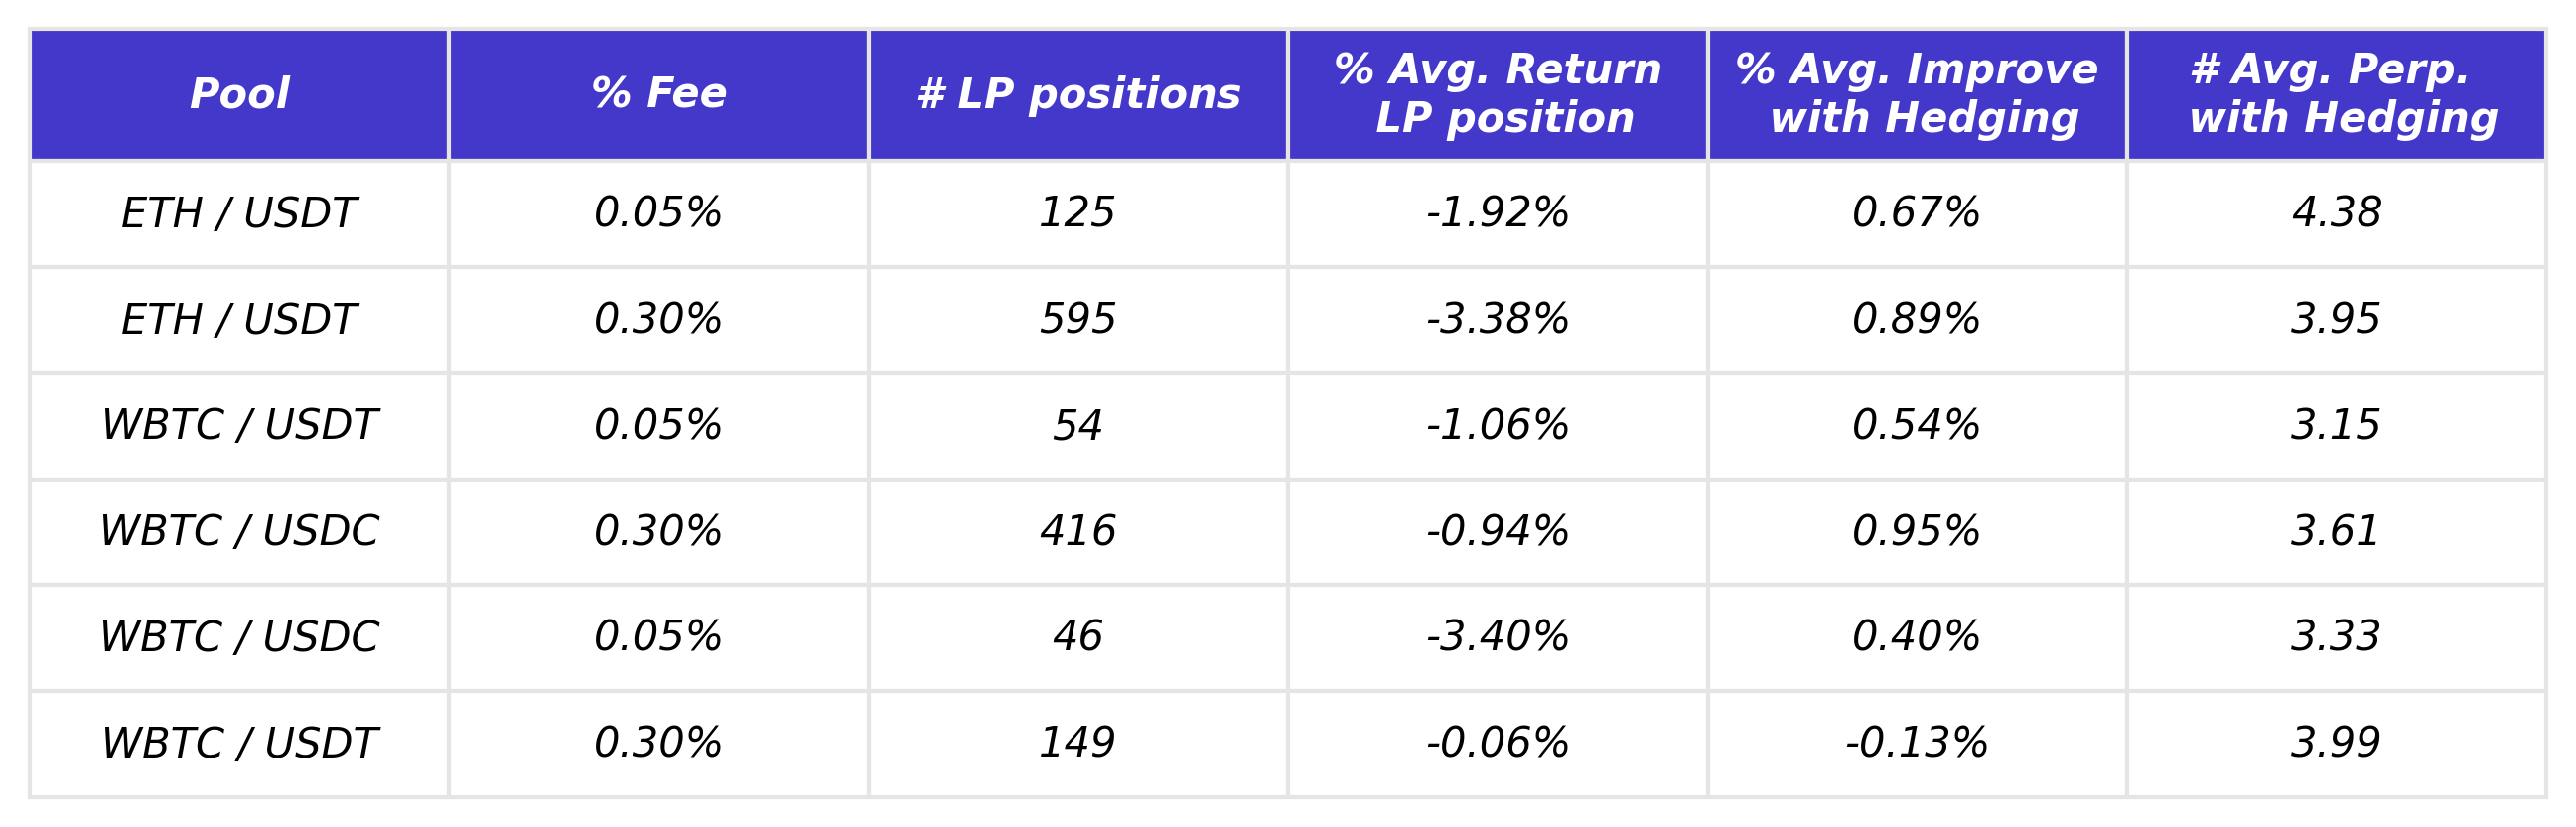
\includegraphics[width=\columnwidth]{img/TblHedge}
\captionof{figure}{Hedging Impact by Pool}
\label{fig:TblHedge}
\justifying
\medskip

Takeaways:
\begin{itemize}
	\item \textbf{Average Returns of LP Positions}: Most pools exhibited negative average returns, ranging from -3.40\% (WBTC/USDC, 0.05\% fee) to -0.906\% (WBTC/USDT, 0.30\% fee). This underperformance is primarily attributed to impermanent loss (IL), a common challenge for LP positions in volatile markets.
	\item \textbf{Average Return Improvement with Hedging}: Hedging consistently improved returns across nearly all pools, with improvements ranging from 0.4\% (WBTC/USDC, 0.05\% fee) up to 1.0\% (ETH/USDT, 0.30\% fee). Collectively, this translated to an additional profit of 1,313k USD across all positions, underscoring the effectiveness of the hedging strategy.
	\item \textbf{Median APY Improvement with Hedging}: The median annual percentage yield (APY) improvement across all pools was approximately 30.87\%. Notably, the WBTC/USDC pool at a 0.300\% fee tier achieved the highest median APY improvement of 60.68\%, while the WBTC/USDC pool at a 0.05\% fee tier showed the lowest at 9.88\%. 
	\item \textbf{Average Number of Perpetual Futures per Position}: On average, each LP position was hedged 3 to 4 times during its lifetime, with values ranging from 3.15 (WBTC/USDT, 0.05\% fee) to 4.38 (ETH/USDT, 0.05\% fee). This frequency reflects the dynamic nature of the hedging strategy, which adjusts to market conditions to mitigate IL.
\end{itemize}


\centering
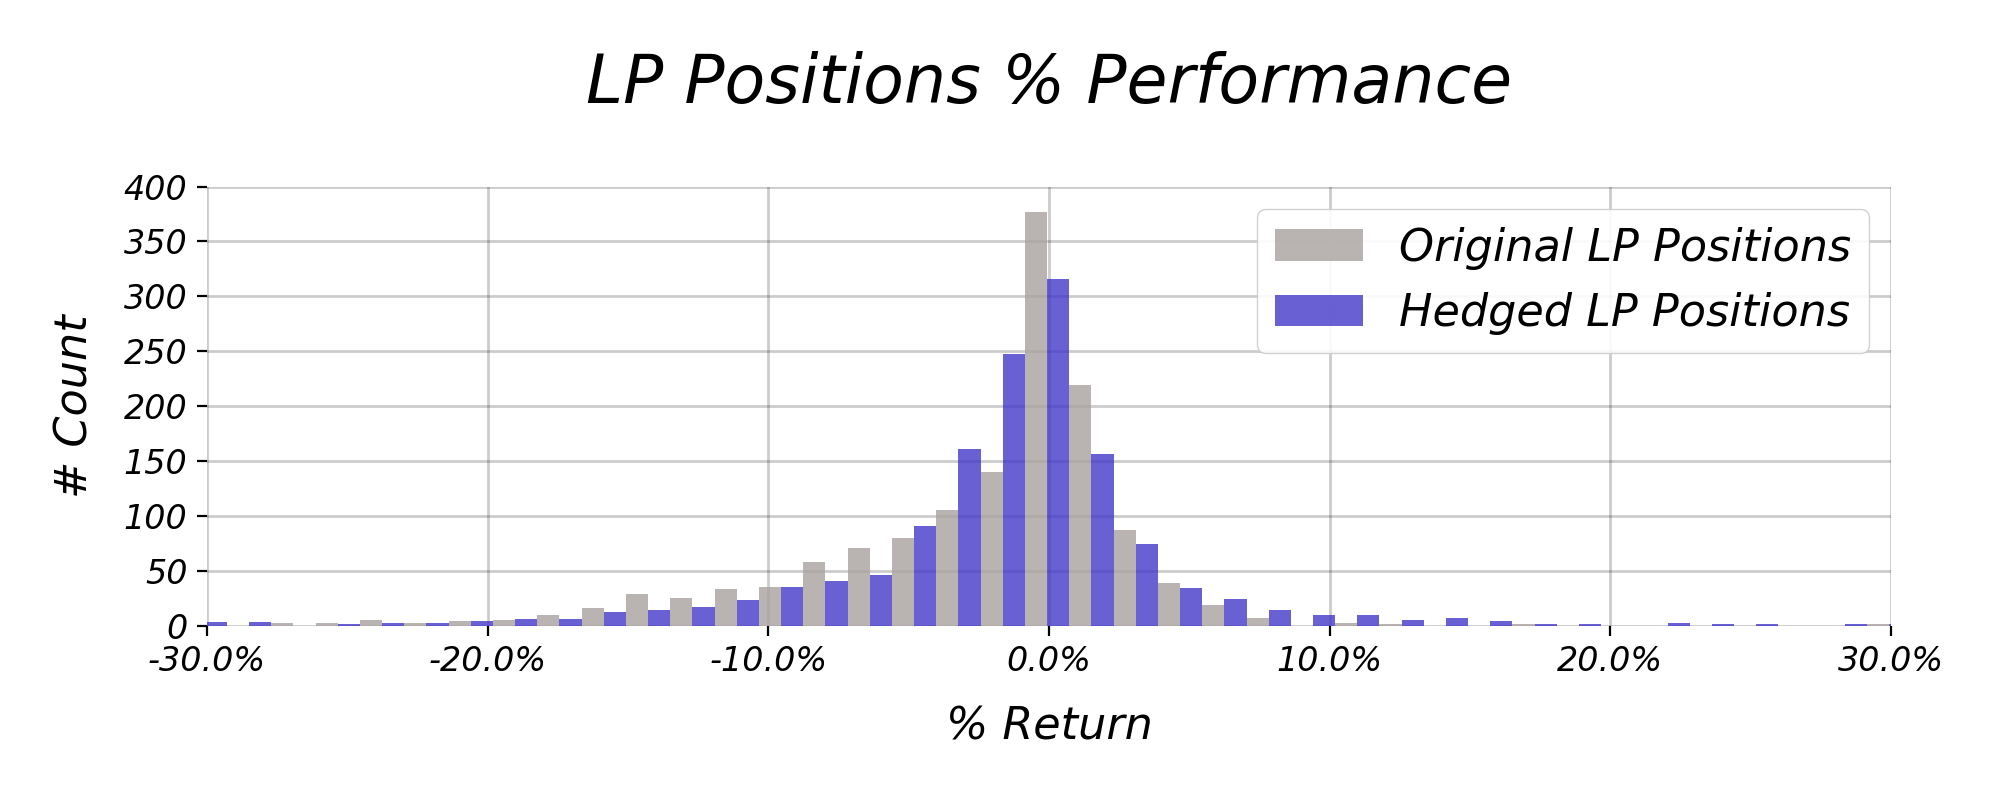
\includegraphics[width=\columnwidth]{img/HistogramPerformance}
\captionof{figure}{Histogram of LP Positions Performance}
\label{fig:HistogramPerformance}
\justifying
\medskip

\centering
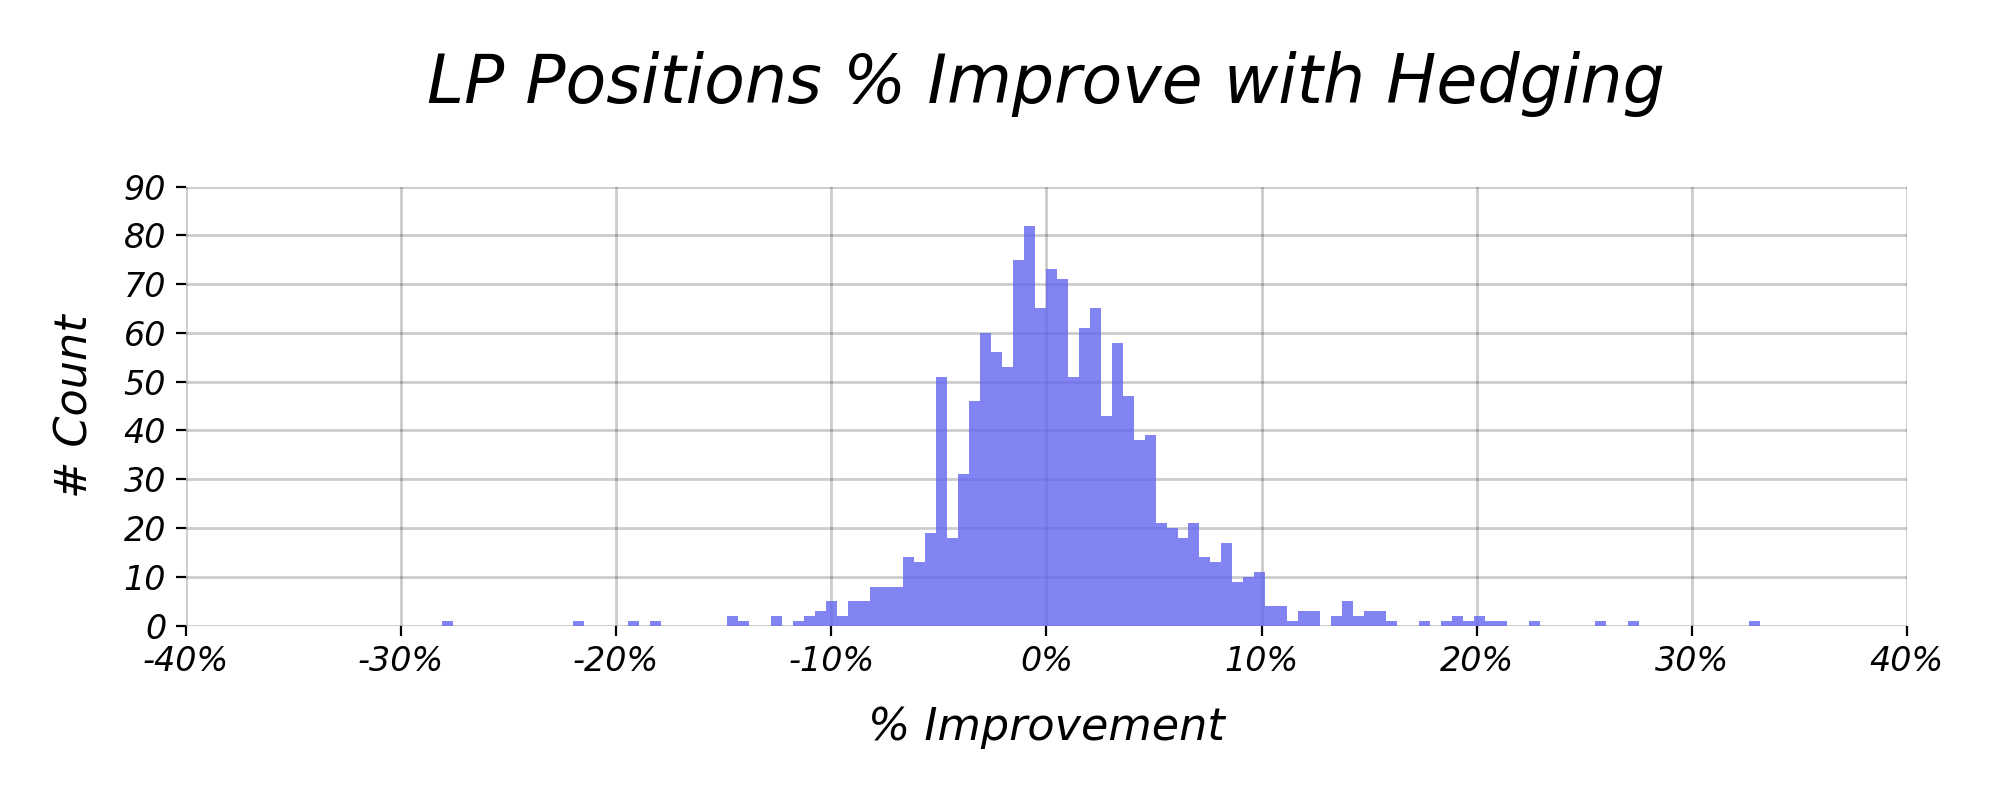
\includegraphics[width=\columnwidth]{img/HistogramImprovement}
\captionof{figure}{Histogram of Improve LP Positions}
\label{fig:HistogramImprovement}
\justifying
\medskip

\subsubsection{Perpetuals by Market State}
\centering
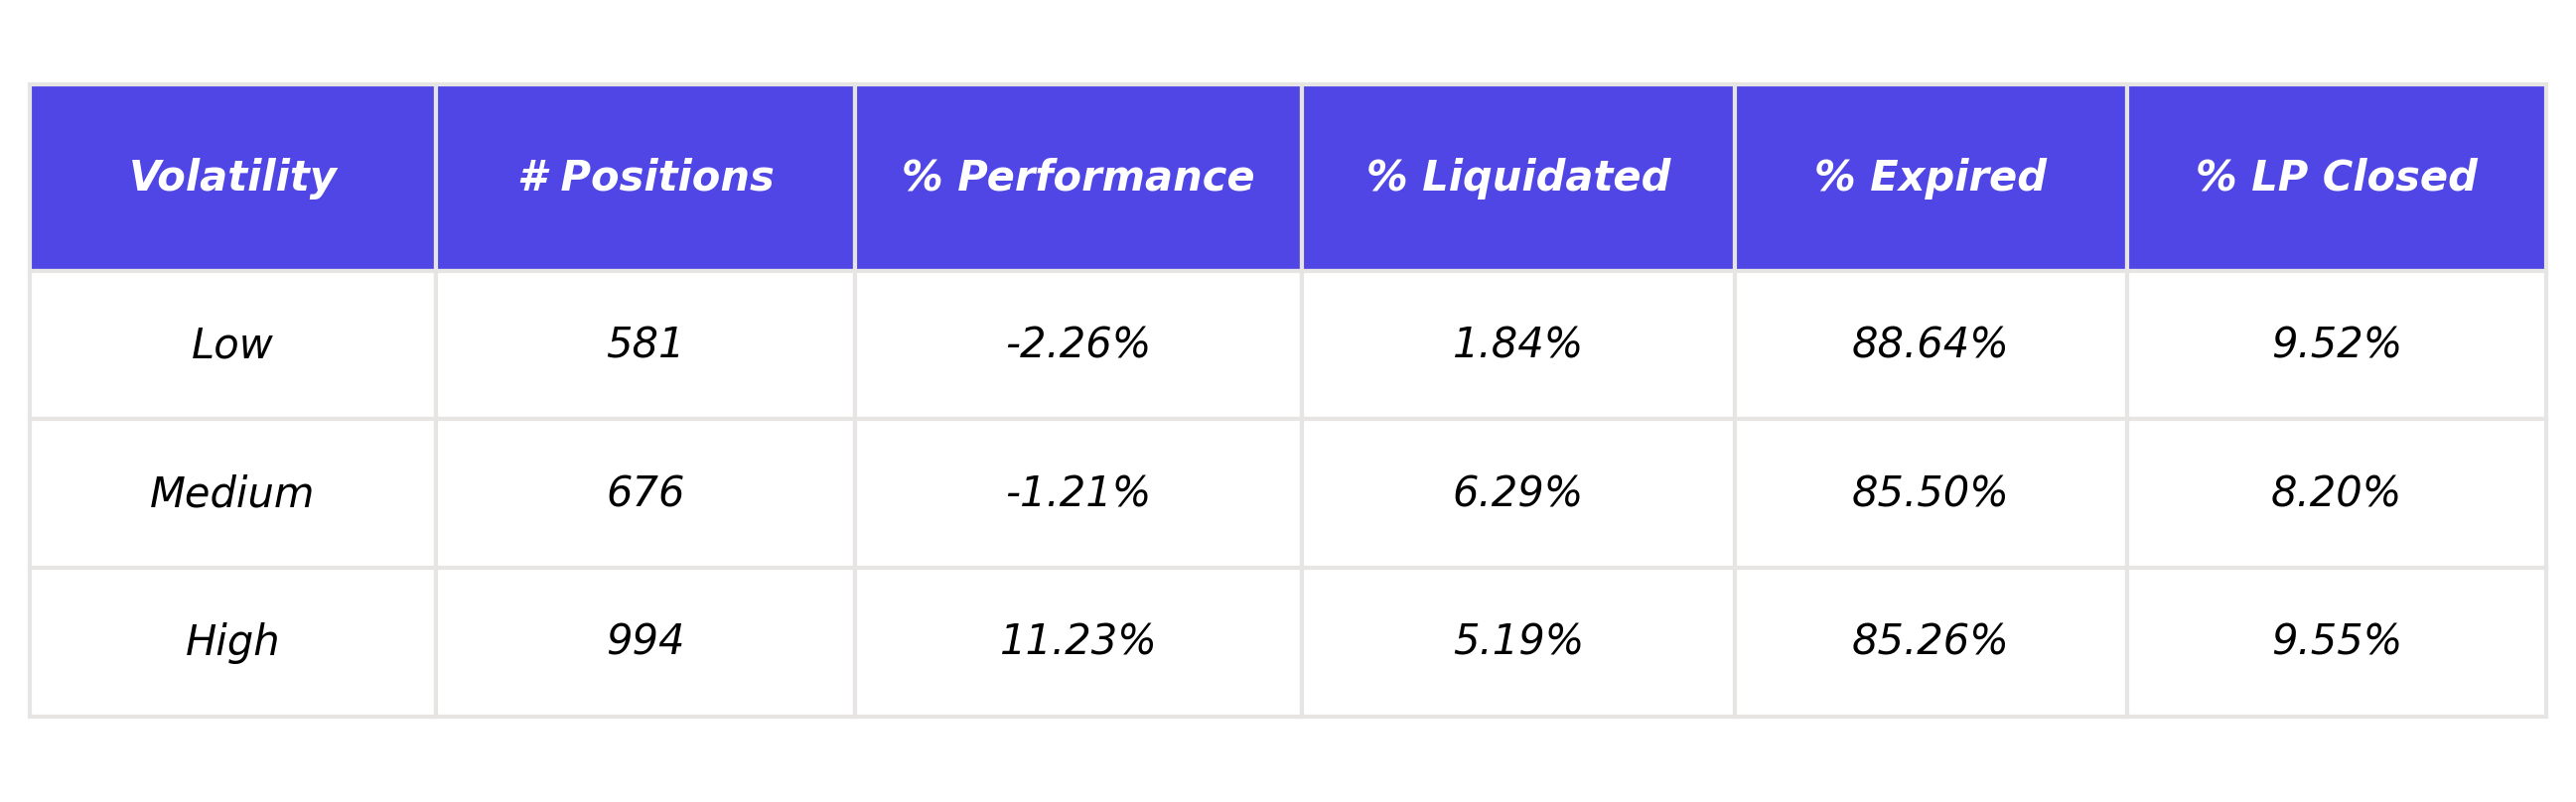
\includegraphics[width=\columnwidth]{img/TblPerps}
\captionof{figure}{Perpetuals Performance by Market State}
\label{fig:TblPerps}
\justifying
\smallskip
The property of avoiding liquidations has been achieved with healthy levels of leverage and duration:

\begin{itemize}
	\item \textbf{\# Positions}: There is sufficient number of perpetuals across market states, with dominating high volatility.
	\item \textbf{\% Performance}: Hedging with perpetuals does not aim for performance but to off-balance the IL. However, there was particularly good performance in high volatility scenarios\footnote{This phenomenon will be inspected in the future to determine possible more speculative and protecting strategy while using perpetuals to hedge positions.}.
	\item \textbf{Closing Perpetuals}:

	\smallskip
	\textbf{\% Liquidated}: the share of liquidated perpetuals is minimal which is an effect of safe leverage driven by Xtreamly Forecasts. 

	\smallskip
	\textbf{\% Expired}: the principal reason for closing perpetuals. While funding rates are the only one limitation to extend perpetual lifetime, navigating through 

	\smallskip
	\textbf{\% LP Closed}: remains in around 10\% level and it is determined only by LP owners actions.

\end{itemize}

\centering
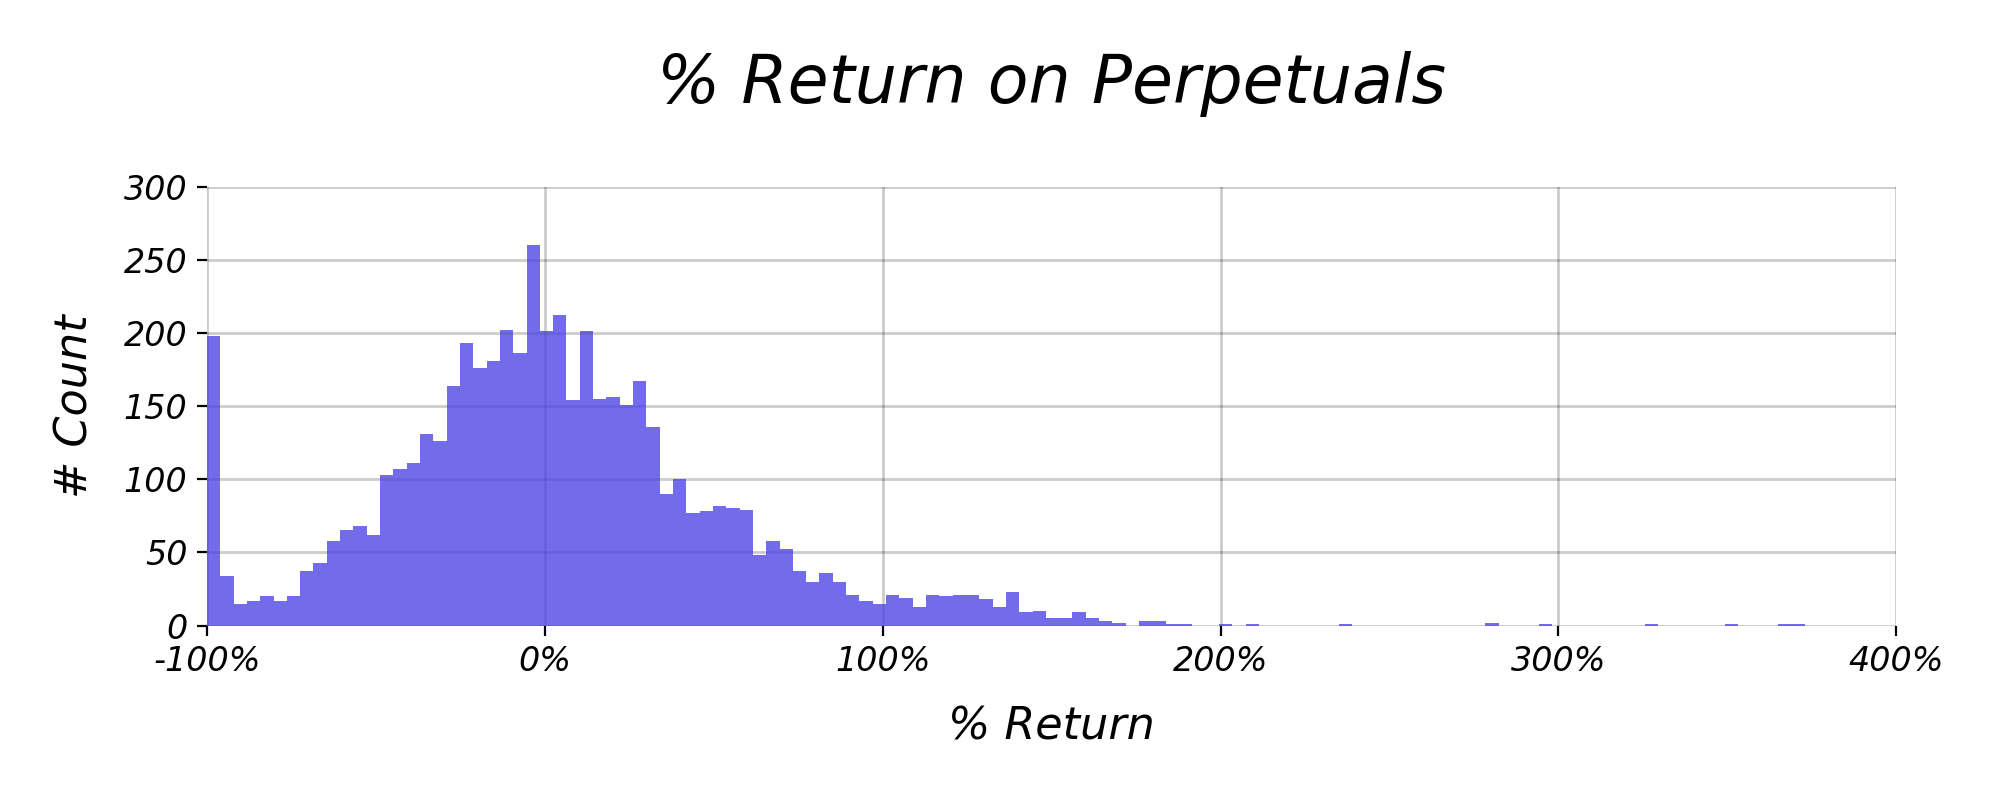
\includegraphics[width=\columnwidth]{img/HistogramReturnPerpetuals}
\captionof{figure}{Histogram of Perpetuals \% Returns}
\label{fig:HistogramReturnPerpetuals}
\justifying

\centering
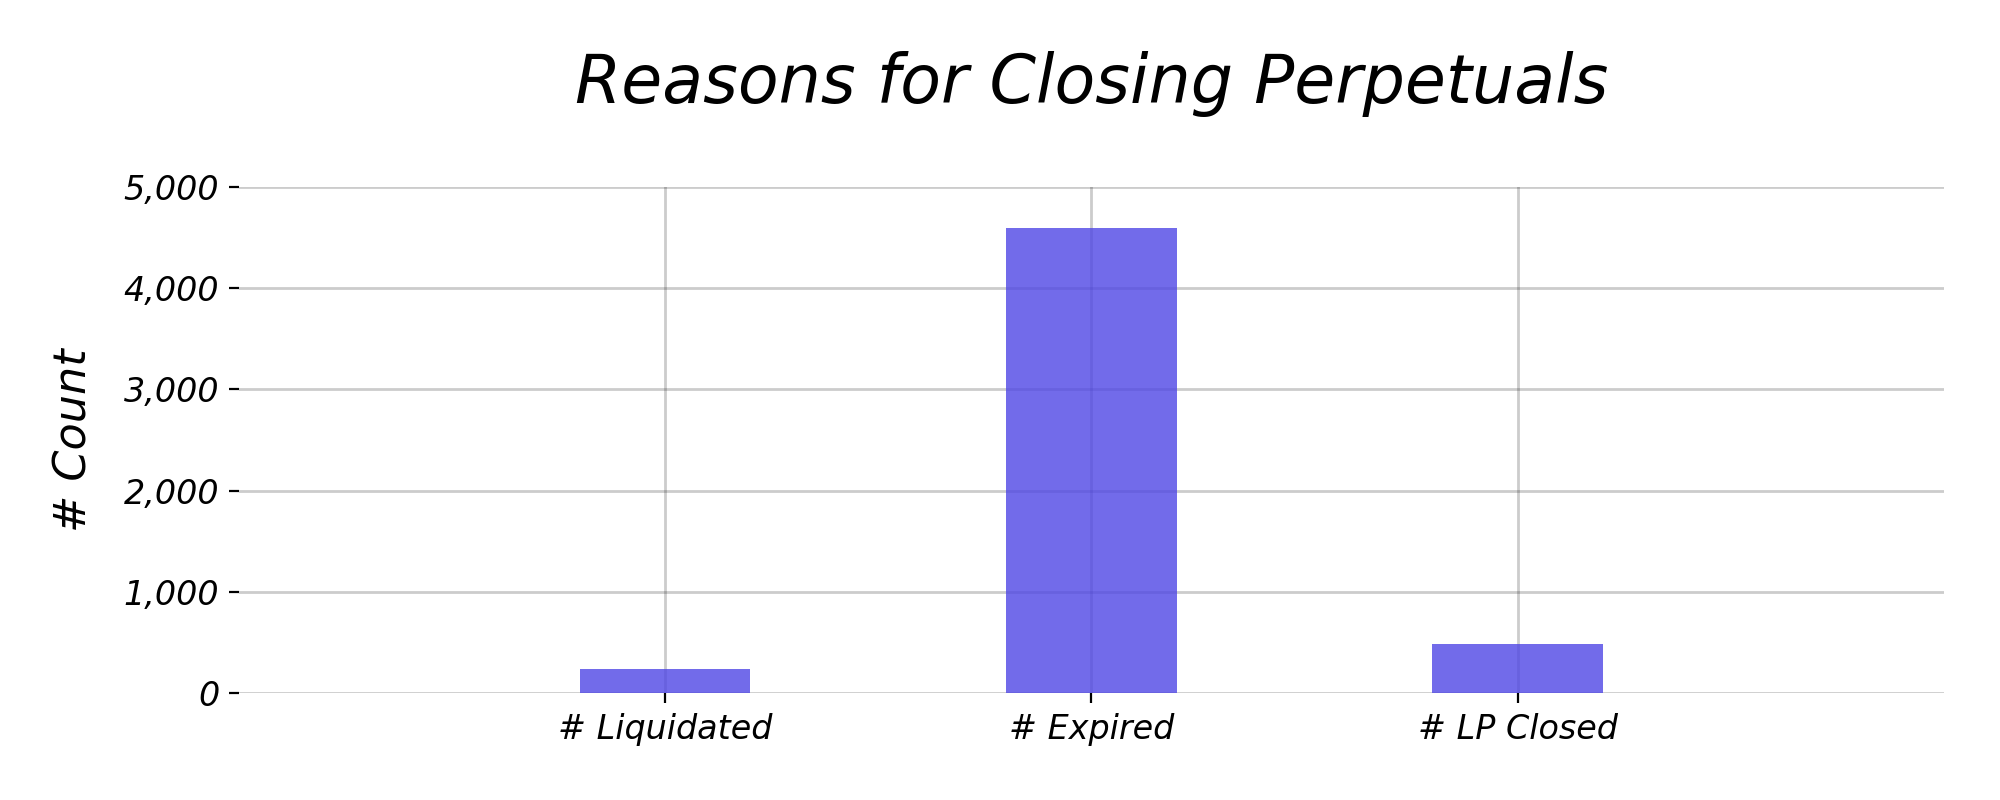
\includegraphics[width=\columnwidth]{img/BarClosePerpetuals}
\captionof{figure}{Bar on Reasons of Closing Perpetuals}
\label{fig:BarClosePerpetuals}
\justifying

\bigskip
\bigskip
\bigskip
\columnbreak
\subsubsection{Hedging Examples}

\justifying
\paragraph{Example 1}

\centering
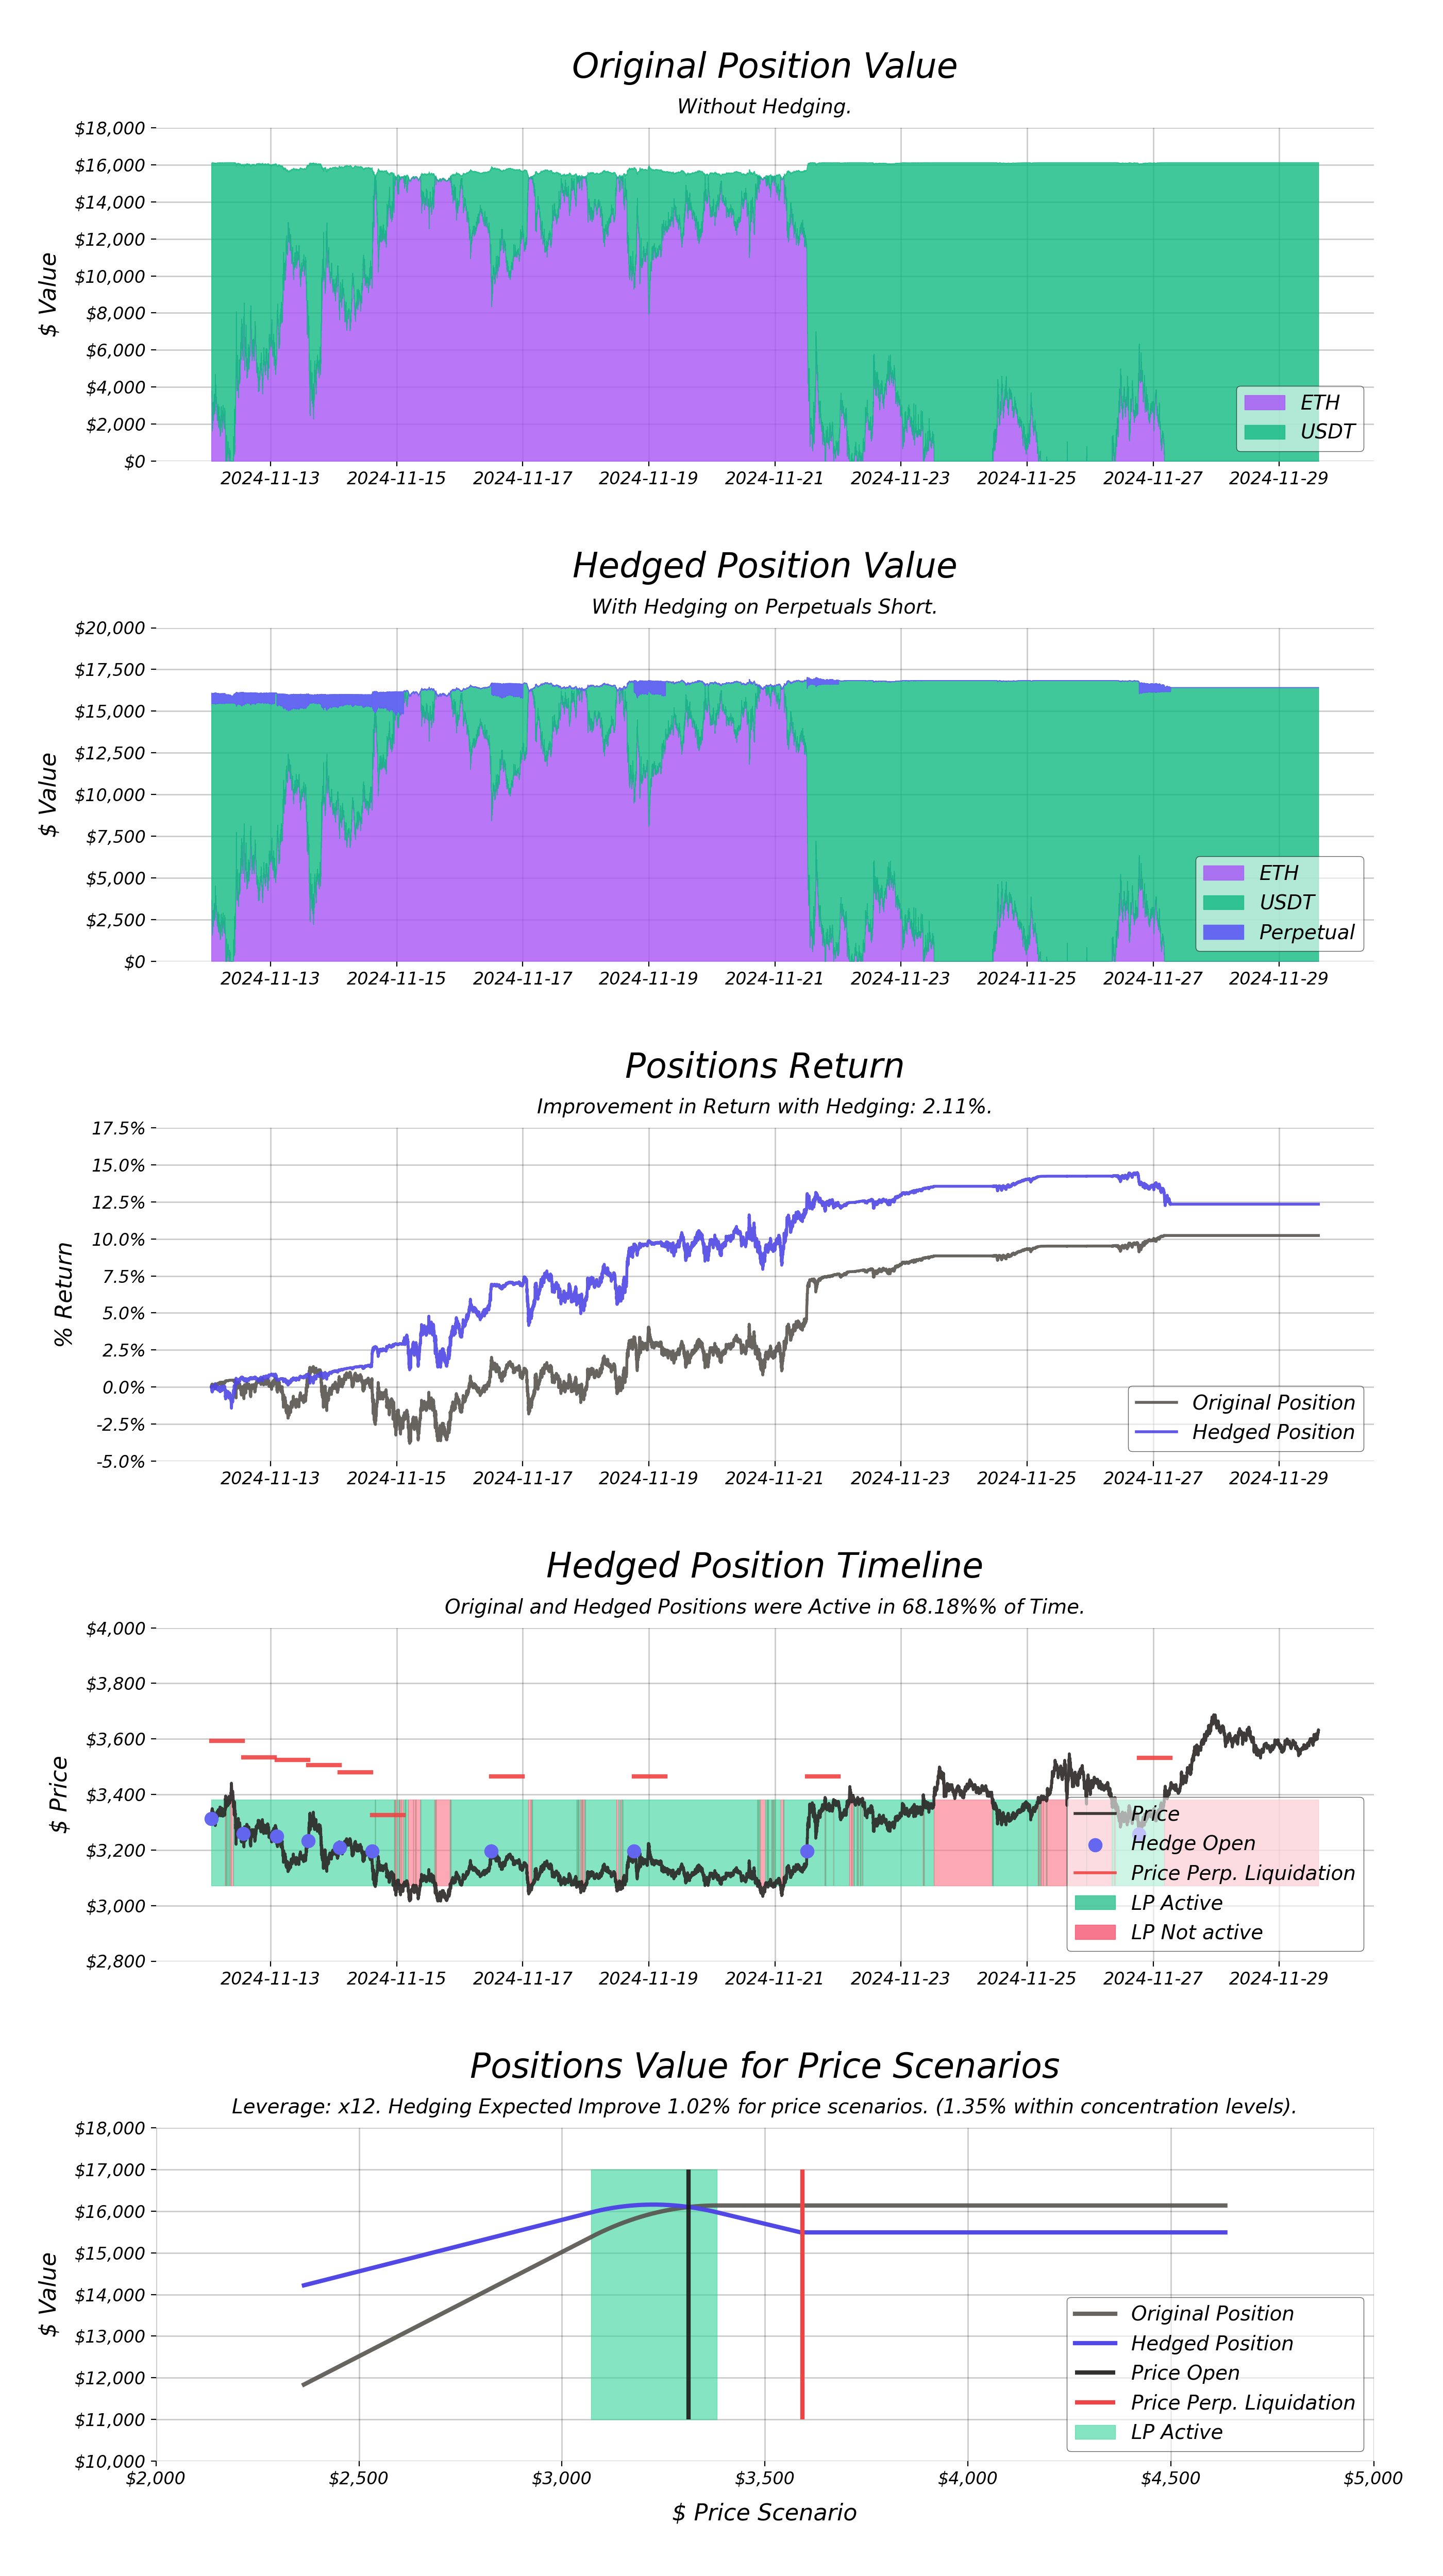
\includegraphics[width=\columnwidth]{img/Position Hedge 855758_0x2b64521c30e63991908bba64e127305ede82fa7b.png}
\captionof{figure}{Example of hedging LP position id: $_{855758_0x2b64521c30e63991908bba64e127305ede82fa7b}$.}
\label{fig:855758_0x2b64521c30e63991908bba64e127305ede82fa7b}
\justifying

\smallskip
\textbf{Hedged Position}: The collateral is a fraction of the LP position to minimize negative impact to LP return.

\smallskip
\textbf{Return}: The hedged position outperforms, despite number of unprofitable hedging and positive price change.

\smallskip
\textbf{Timeline}: The hedging with short perpetuals has been done over 10 times, with different leverage levels. 

\smallskip
\textbf{Payoff Value}: For uniform uniform distribution of price scenarios, the expected return of hedged position is greater than original position. 

\columnbreak

\paragraph{Example 2}

\smallskip
\centering
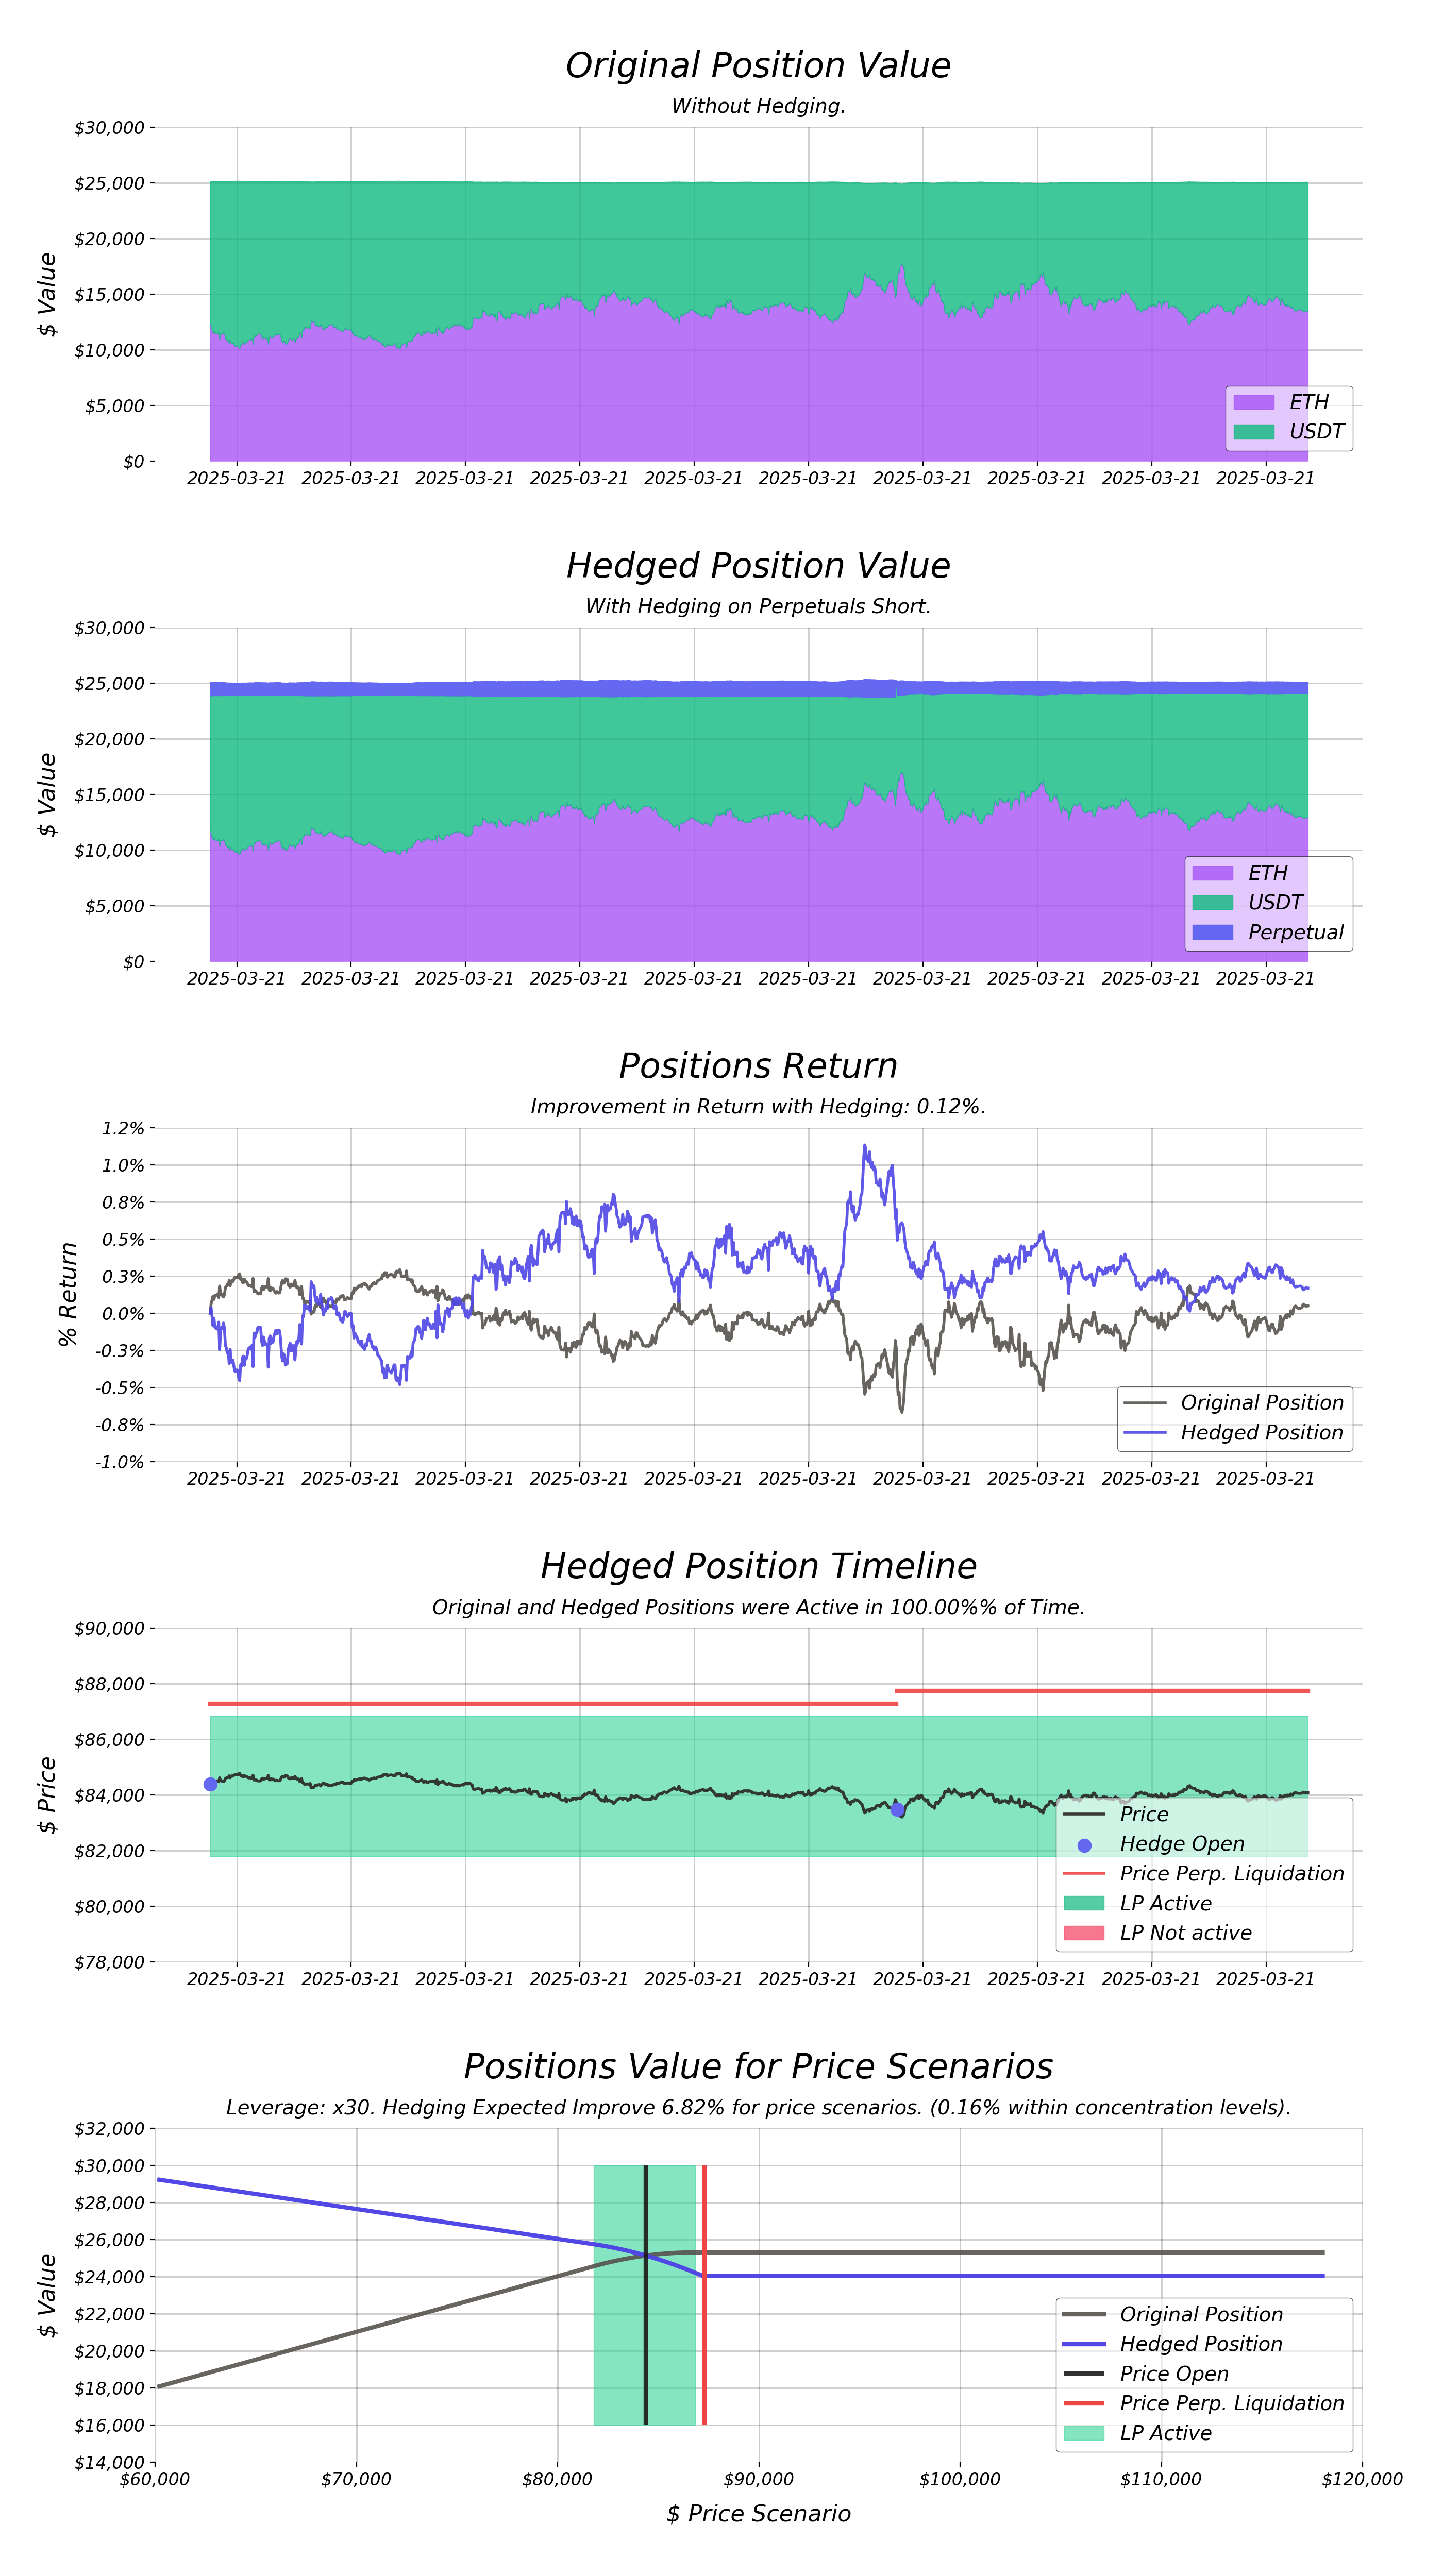
\includegraphics[width=\columnwidth]{img/Position Hedge 951878_0x51a56768dd4d255e9c9993d03100d3d10541f4e7.png}
\captionof{figure}{Example of hedging LP position id: $_{951878_0x51a56768dd4d255e9c9993d03100d3d10541f4e7}$.}
\label{fig:951878_0x51a56768dd4d255e9c9993d03100d3d10541f4e7}
\justifying

\medskip
\textbf{Hedged Position}: The perpetual is active during the LP position lifetime

\smallskip
\textbf{Return}: The hedged position reversed the return due to downgrading price and increased leverage.

\smallskip
\textbf{Timeline}: Liquidation price is kept in safe levels despite x30 leverage.

\smallskip
\textbf{Payoff Value}: The expected return of hedged position is greater than original position for full scope of price scenarios. 

\bigskip
\bigskip
\bigskip

\section{DeFi Implementation}

\subsection{Hook Deployment}
Our Uniswap V4 hook implements an event-driven hedging infrastructure through custom \textit{afterAddLiquidity()} and \textit{afterRemoveLiquidity()} functions. The workflow encompasses:
\begin{enumerate}
	\item \textbf{Event Emission}: Hook generates detailed events on LP position changes.
	\item \textbf{Webhook Trigger}: Backend webhook captures these events.
	\item \textbf{Position Data Query}: Comprehensive position data retrieval.
	\item \textbf{Hedging Decision}: Algorithmic strategy determination.
	\item \textbf{Execution}: Off-chain infrastructure creates increase orders on target protocols.
\end{enumerate}

\subsection{Protocol Ecosystem}
We target GMX V2 as the primary hedging protocol, with plans to expand into Opyn Markets, Derive Markets, and additional DeFi hedging mechanisms. This multi-protocol approach diversifies hedging strategies, optimizes risk management, and provides flexible liquidity solutions.

\subsection{Infrastructure Architecture}
\subsubsection{Data Management}
We employ PostgreSQL with the Timescale extension for optimized time-series data storage, efficient transaction history tracking, and position monitoring. Key storage components include LP position records, hedge transaction logs, protocol interaction metadata, and performance metrics.
\subsubsection{Funding Approach}
Our funding mechanism has dedicated per-user funding wallet generation upon fronted wallet connection, with secure transaction signing infrastructure.

\subsection{Decentralization Strategy}
\subsubsection{Current Infrastructure Characteristics}
The current system is centralized to balance performance and operational efficiency, with a long-term vision of incremental decentralization. This approach systematically reduces central control while preserving system efficiency.

\subsubsection{Multi-signature  Wallet Design}
We have planned multi-signature capabilities include role-based access control, granular protocol interaction permissions, dynamic liquidity management, and cross-protocol transaction authorization.

\subsubsection{Future Hook Capabilities}
Future development targets implementing role-based access control for hook modifications, enabling dynamic cross-user liquidity management, supporting flexible fee structures, and creating sophisticated cross-protocol hedge strategies. Proposed multi-signature functions will cover protocol-specific contract interactions, dynamic liquidity rebalancing, fee structure modifications, and hedge strategy execution across platforms.

\subsubsection{Uniswap V4 Interaction Constraints}
While Uniswap V4 currently limits external liquidity modifications, our roadmap includes developing advanced hook mechanisms to implement access controls, enable authorized third-party liquidity management, and create more flexible liquidity provision models.

\section{Further Work}
\label{sec:futurework}

\subsection{Further Analysis}
Future research should extend the analysis to a broader range of pools and timelines. This will further validate the strategy’s robustness across various scenarios, including bull and bear markets, and periods of different volatility.

\subsection{Forecasting Enhancements}
Integrating Xtreamly’s AI predictive methodology to the intelligence behind opening and closing perpetual positions, in particular:
\begin{itemize}
	\item \textbf{Maximum Drawdown and Drawup}: to enhance leverage that minimize liquidation risk. 
	\item \textbf{Semivariance}: to asses risk a specific direction and optimize collateral allocation and tailor hedges to directional risks, improving capital efficiency.
	\item \textbf{Price}: to add speculative component of directional risks, improving capital efficiency.
	\item \textbf{Funding Rate Prediction}: Predict funding rates to extend the maximum holding time of perpetual positions, reducing the impact of funding costs on hedging profitability.
	\item \textbf{Dynamic Fee Prediction}: Predict Uniswap’s dynamic fees to optimize collateral cost for hedging, by balancing the trade-off between future collected fees and IL. This means, whenever higher collected fees are predicted, the IL is less material. 
\end{itemize}

\subsection{AI-Driven Hedging Signals}
Leverage Xtreamly’s AI predictions to identify additional timing for additional hedging actions. In particular, the system could detect periods with a high likelihood of significant price drops, signaling the need for increased short perpetual exposure.

\subsection{AI-Agent}
Develop an automated investment agent that would combine all of the hedging rules, and with additional capability to self manage perpetual exposure and rebalancing LP positions. This agent will:
\begin{itemize}
	\item \textbf{Rebalance LP positions} by reallocating liquidity across price ranges to keep LP position active.
	\item \textbf{Hedge LP positions} by monitoring real-time market data, adjusting perpetual leverage and notional size to maximize returns.
\end{itemize}
Such automation would reduce manual intervention, increase scalability, and ensure consistent strategy execution. 

\subsection{Hedging with Options}
Integration of DeFi options trading via platforms like Panoptic to complement perpetual-based hedging. Options could secure protection during high-volatility periods, in particular: using put options to hedge against downside IL when prices drop below 

\medskip

This approach would diversify hedging tools, potentially reducing reliance on leverage and funding costs while enhancing protection in extreme market conditions.

\newpage

\section{Appendix}

\bigskip

\subsection{Hedging Mathematics}
\medskip
\subsubsection{LP Position}
Let's consider LP variables:

\begin{itemize}
	\item $P$: The current market price
	\item $P_L$: The lower bound price
	\item $P_U$: The upper bound price
	\item $L$: The \emph{constant} liquidity of the LP position
	\item $X_0$: The amount of $token_0$ held at LP opening
	\item $Y_0$: The amount of $token_1$ held at LP opening
\end{itemize}

\textbf{Ignoring fees}: We assume the LP payoff depends only on the realized price $P$.

\subsubsection{Three Cases for the LP Value}

\paragraph{Case 1: Within Range} $P_L \le P \le P_U$
 
\smallskip

When the market price $P$ lies within the chosen range $[P_L, P_U]$, the position consists of a mix of $token_0$ and $token_1$. The exact amounts of each asset are determined by Uniswap's liquidity formula of $P$:

\begin{align*}
X(P) = L \biggl(\frac{1}{\sqrt{P}} - \frac{1}{\sqrt{P_U}}\biggr)
\end{align*}
\begin{align*}
Y(P) = L \bigl(\sqrt{P} - \sqrt{P_L}\bigr)
\end{align*}

where:
\begin{itemize}
	\item $L$ is the total liquidity provided to the range.
	\item $X(P)$ represents the amount of $token_0$.
	\item $Y(P)$ represents the amount of $token_1$.
\end{itemize}

The LP total value is the value of both tokens:
\[
V_{\text{Case 1}}(P) = X(P) \cdot P \;+\; Y(P).
\]

Expanding:
\begin{align*}
V_{\text{Case 1}}(P) &= L \biggl(\frac{1}{\sqrt{P}} - \frac{1}{\sqrt{P_U}}\biggr) P \\
&\quad + L \bigl(\sqrt{P} - \sqrt{P_L}\bigr),
\quad \text{for } P_L \le P \le P_U.
\end{align*}

\paragraph{Case 2: Below Range} $P < P_L$.
 
\smallskip

When the price drops below $P_L$, the liquidity position has been fully converted into $token_0$. This happens because as price decreases, the Uniswap mechanism sells all available $token_1$ in exchange for $token_0$. So, the $token_0$ amount is locked at the value of $P_L$:
\[
X(P_L) = L \biggl(\frac{1}{\sqrt{P_L}} - \frac{1}{\sqrt{P_U}}\biggr).
\]
The LP holds only $token_0$:
\[
V_{\text{Case 2}}(P) = X(P_L) \cdot P.
\]
Expanding:
\[
V_{\text{Case 2}}(P) = L \biggl(\frac{1}{\sqrt{P_L}} - \frac{1}{\sqrt{P_U}}\biggr) P,
\quad \text{for } P < P_L.
\]

\paragraph{Case 3: Above Range} $P > P_U$.
 
\smallskip

When the price moves above $P_U$, the liquidity position has been fully converted into $token_1$. This happens because as price increases, the Uniswap mechanism sells all available $token_0$ in exchange for $token_1$.

\medskip

The $token_1$ amount is locked at the value it had at $P_U$, which is:
\[
Y(P_U) = L \bigl(\sqrt{P_U} - \sqrt{P_L}\bigr).
\]
The LP holds only $token_1$:
\[
V_{\text{Case 3}}(P) = Y(P_U).
\]
Expanding:
\[
V_{\text{Case 3}}(P) = L \bigl(\sqrt{P_U} - \sqrt{P_L}\bigr),
\quad \text{for } P > P_U.
\]

\paragraph{Final Piecewise Formula.}
 
\smallskip

The complete value function for the LP position is:
\[
V(P) =
\begin{cases}
V_{\text{Case 1}}(P), & \text{for } P < P_L,\\[8pt]
V_{\text{Case 2}}(P), & \text{for } P_L \le P \le P_U,\\[10pt]
V_{\text{Case 3}}(P), & \text{for } P > P_U.
\end{cases}
\]

\smallskip
\centering
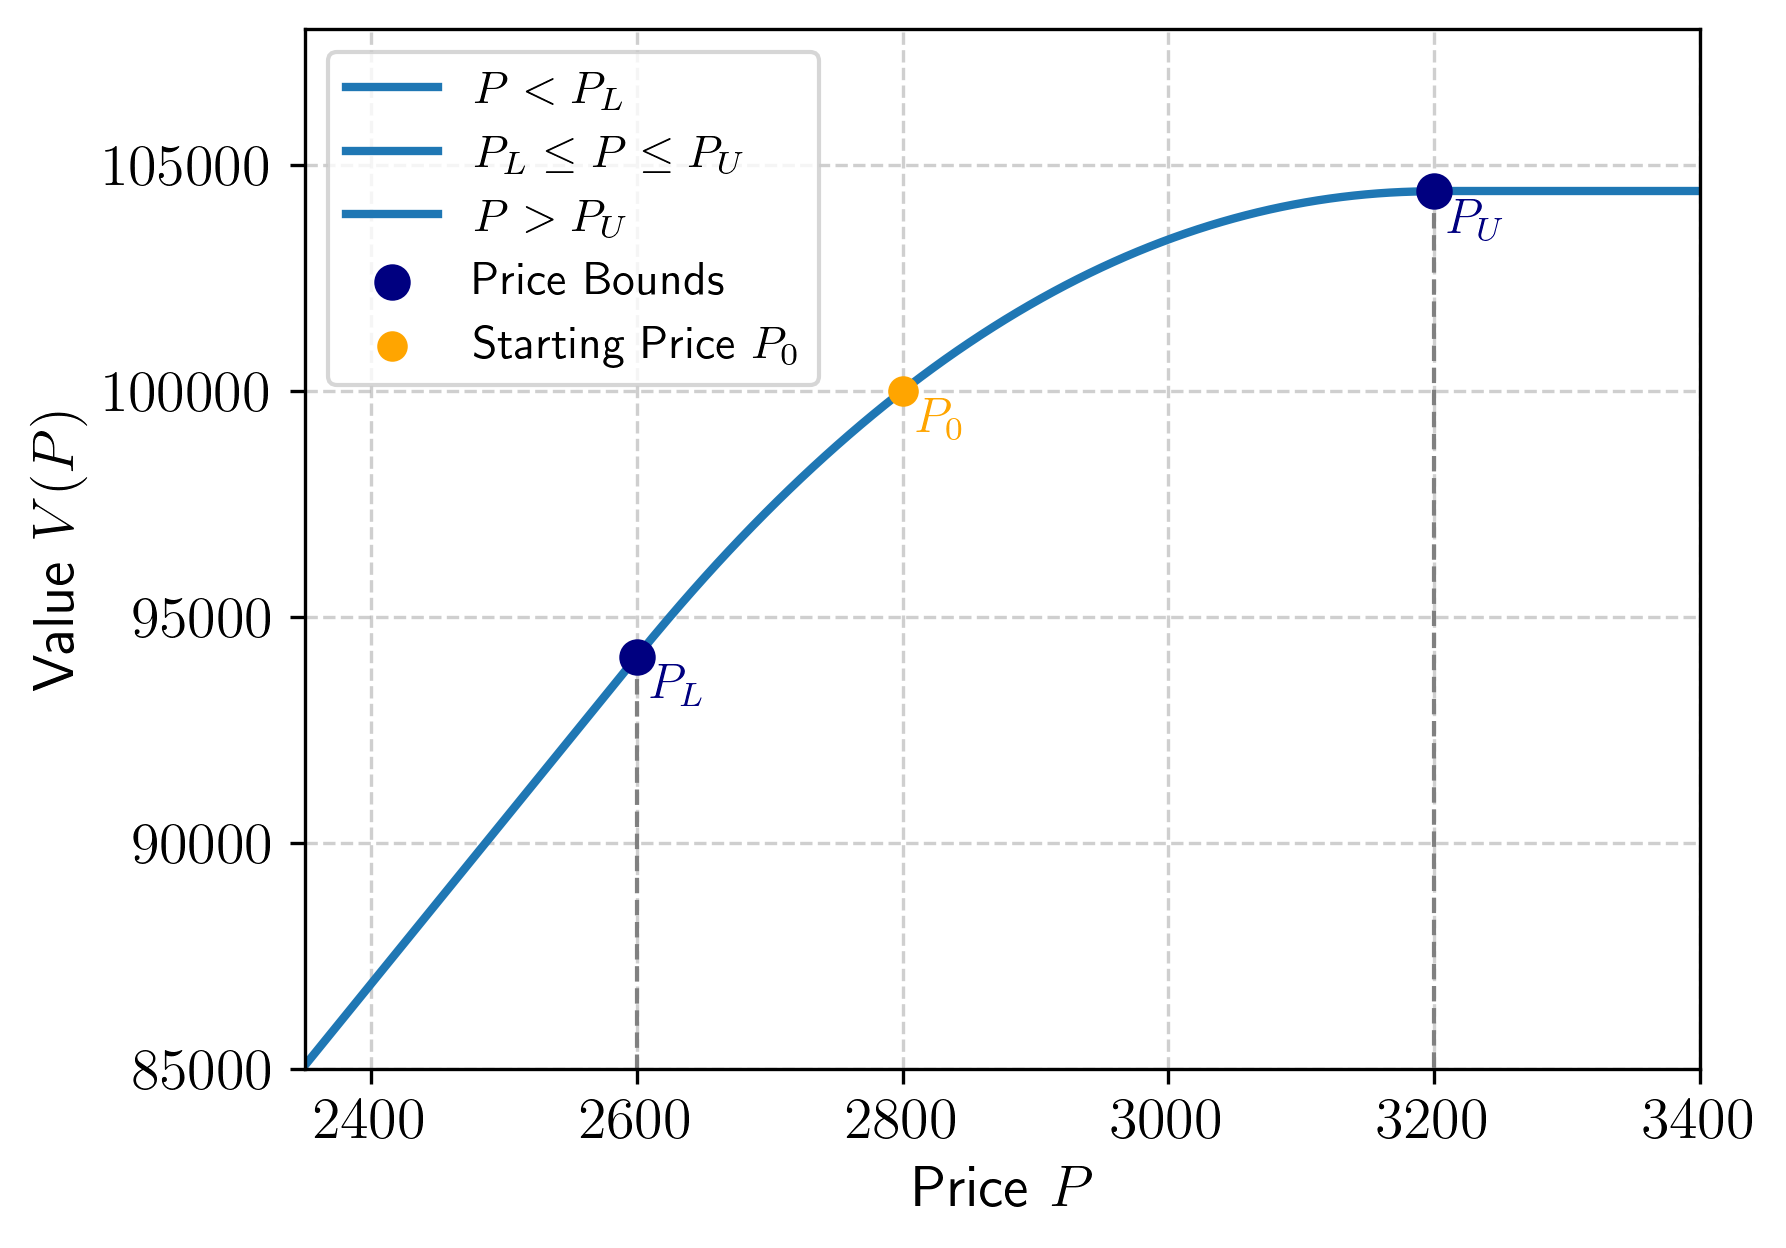
\includegraphics[width=0.9\columnwidth]{img_math/CLposition.png}
\caption{Piece-wise value of a LP position.}
\label{fig:CLposition}
\justifying

\subsubsection{Perpetual Positions}
\label{sec:mathperpetuals}
Let's consider perpetual variables:
\begin{itemize}
	\item $M$: The collateral (in $token_1$) at opening.
	\item $\alpha$: The \emph{notional} size of the perpetual.
	\item $P_0$: The entry price ($token_1$ per $token_0$).
	\item $P_{\mathrm{liq}}$: The liquidation price at which the perpetual is closed and collateral is lost.
\end{itemize}

\paragraph{Short Perpetual}  
 
\smallskip

Suppose we \emph{short} at price $P_0$. The PnL from the short is $\alpha\,(P_0 - P)$. We post margin $M$ to cover losses if $P$ rises. We define $P_{\mathrm{liq}}$ so that when $P = P_{\mathrm{liq}}$, our margin is fully exhausted:
\[
M + \alpha\,(P_0 - P_{\mathrm{liq}}) = 0
\quad\Longrightarrow\quad
P_{\mathrm{liq}} = P_0 + \frac{M}{\alpha}.
\]
Hence, our \textbf{short} payoff is
\[
V_{\mathrm{short}}(P) = 
\begin{cases}
M + \alpha\,(P_0 - P), & P < P_{\mathrm{liq}},\\
-M, & P \ge P_{\mathrm{liq}}.
\end{cases}
\]

\smallskip
\centering
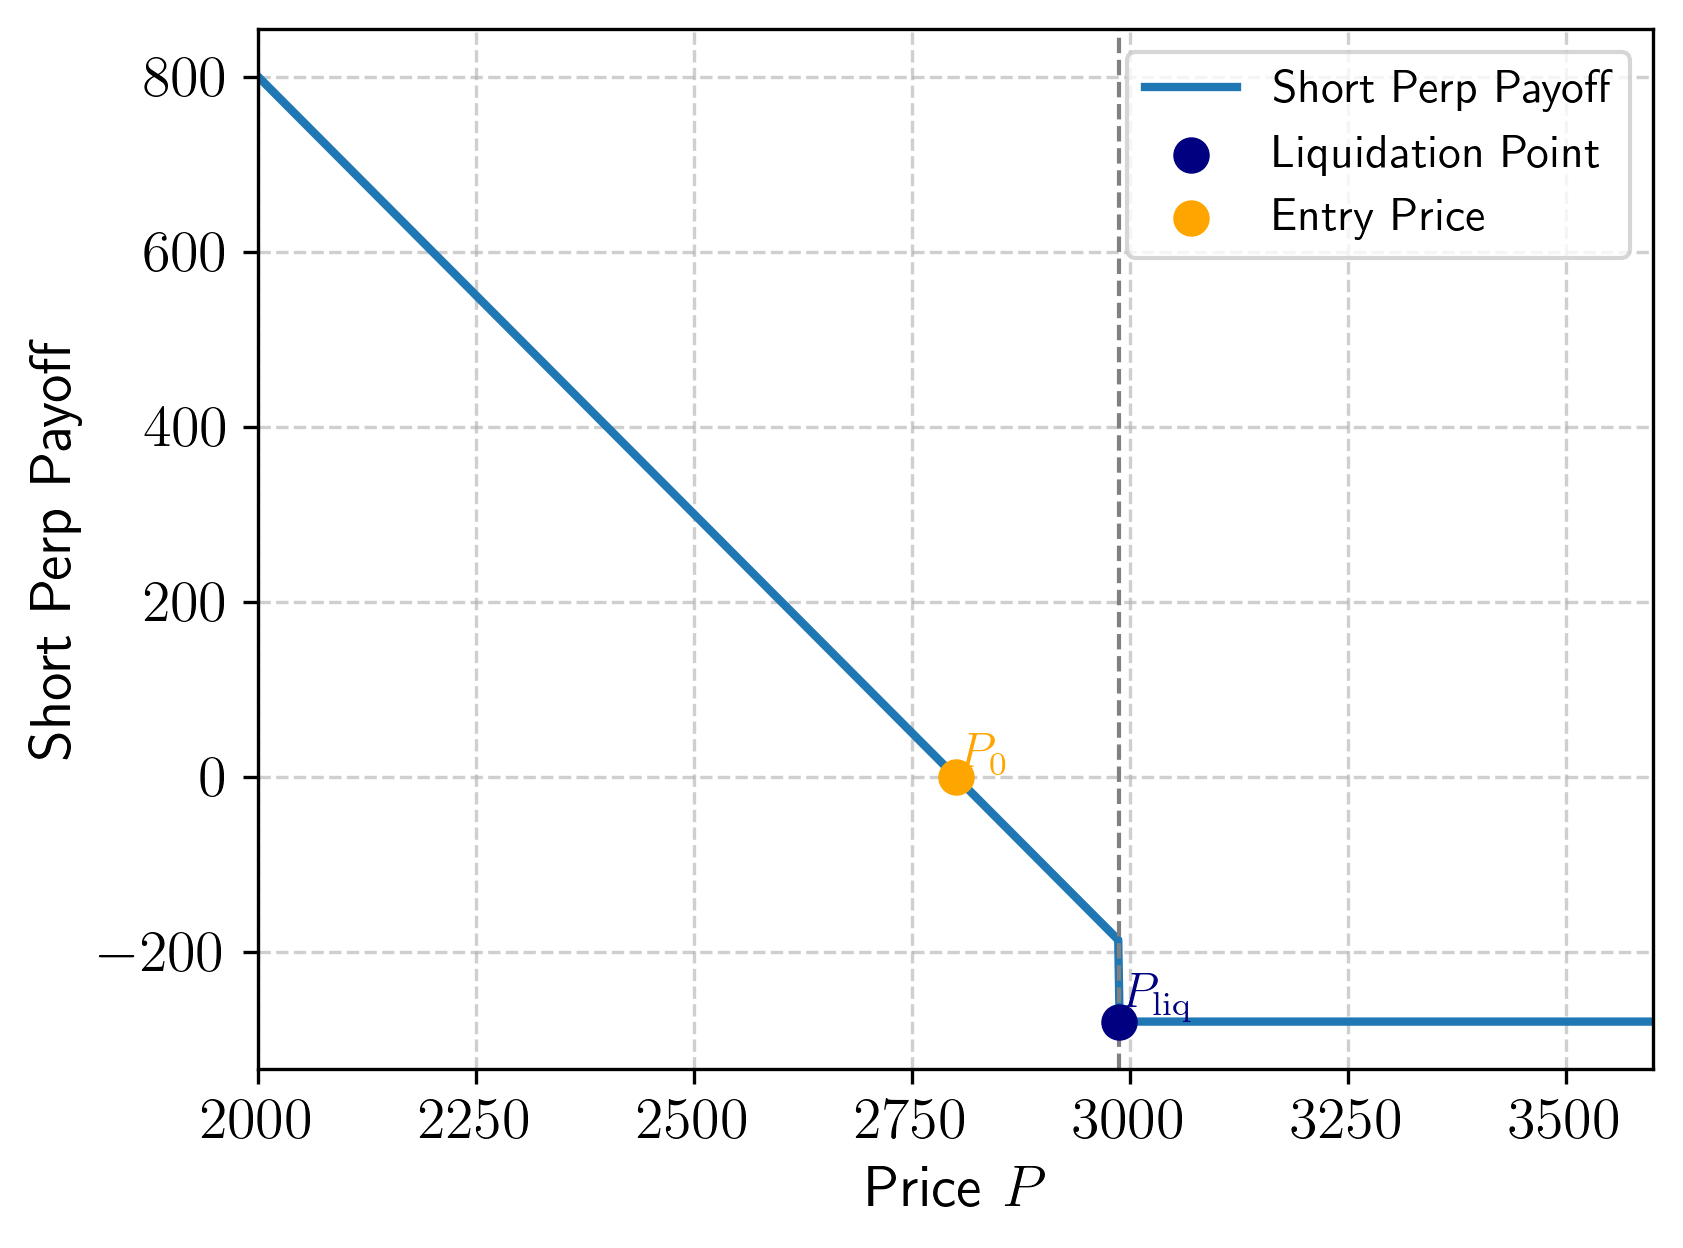
\includegraphics[width=0.9\columnwidth]{img_math/short.png}
\captionof{figure}{Piecewise payoff for the Short Perpetual, showing the drop to $-M$ at liquidation.}
\label{fig:short}
\justifying
\medskip

\paragraph{Long Perpetual}  
 
\smallskip

If we \emph{long} at $P_0$, the PnL is $\alpha\,(P - P_0)$. The margin $M$ is depleted if $P$ falls by enough. Setting $P = P_{\mathrm{liq}}$ where margin is exhausted:
\[
M + \alpha\,(P_{\mathrm{liq}} - P_0) = 0
\quad\Longrightarrow\quad
P_{\mathrm{liq}} = P_0 - \frac{M}{\alpha}.
\]
Hence, our \textbf{long} payoff is
\[
V_{\mathrm{long}}(P) = 
\begin{cases}
-M, & P \le P_{\mathrm{liq}},\\
\alpha\,(P - P_0), & P > P_{\mathrm{liq}}.
\end{cases}
\]

At liquidation ($P = P_{\mathrm{liq}}$), the payoff \emph{jumps} from some positive level (on the linear portion) down to $-M$, reflecting full loss of the margin. This discontinuous drop represents the complete loss of collateral at the liquidation boundary.

\smallskip
\centering
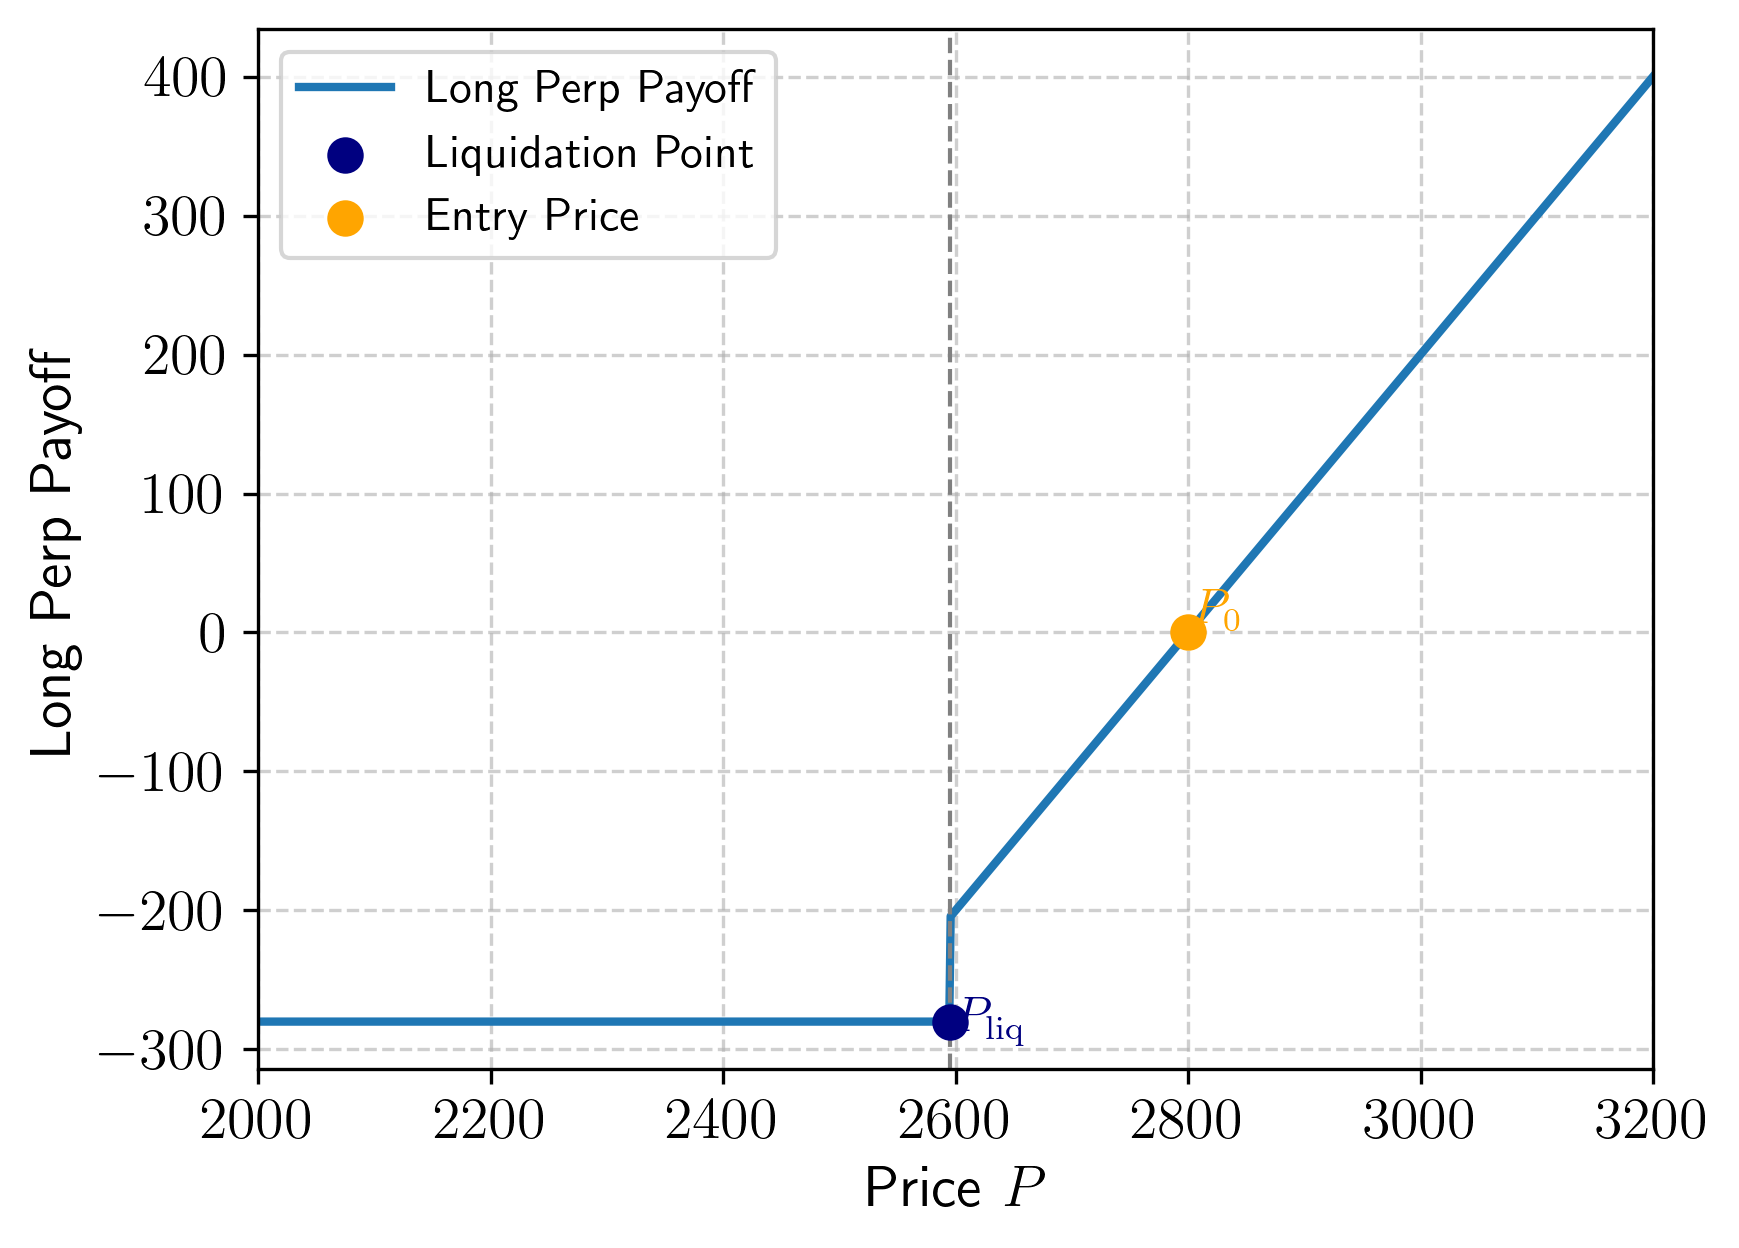
\includegraphics[width=0.9\columnwidth]{img_math/long.png}
\caption{Piece-wise payoff for the Long Perpetual, showing the drop to $-M$ at liquidation.}
\label{fig:long}
\justifying
\medskip

\newpage


\subsection{Alternative Strategies}
\label{sec:alternative}

This section explores alternative combinations of an LP position with perpetual hedges and highlights their potential applications.

\medskip
However, these strategies retain the inherent risks of perpetual positions. For instance, if the price oscillates frequently around the entry levels of the perpetual positions, liquidations may occur before meaningful profits are realized. This could lead to accumulated losses, undermining the hedges’ intended purpose of managing long-term exposure.

\subsubsection{Multi Short Perpetual Strategy}

The single short perpetual hedging strategy was discussed in Section~\ref{sec:hedging}.

\centering
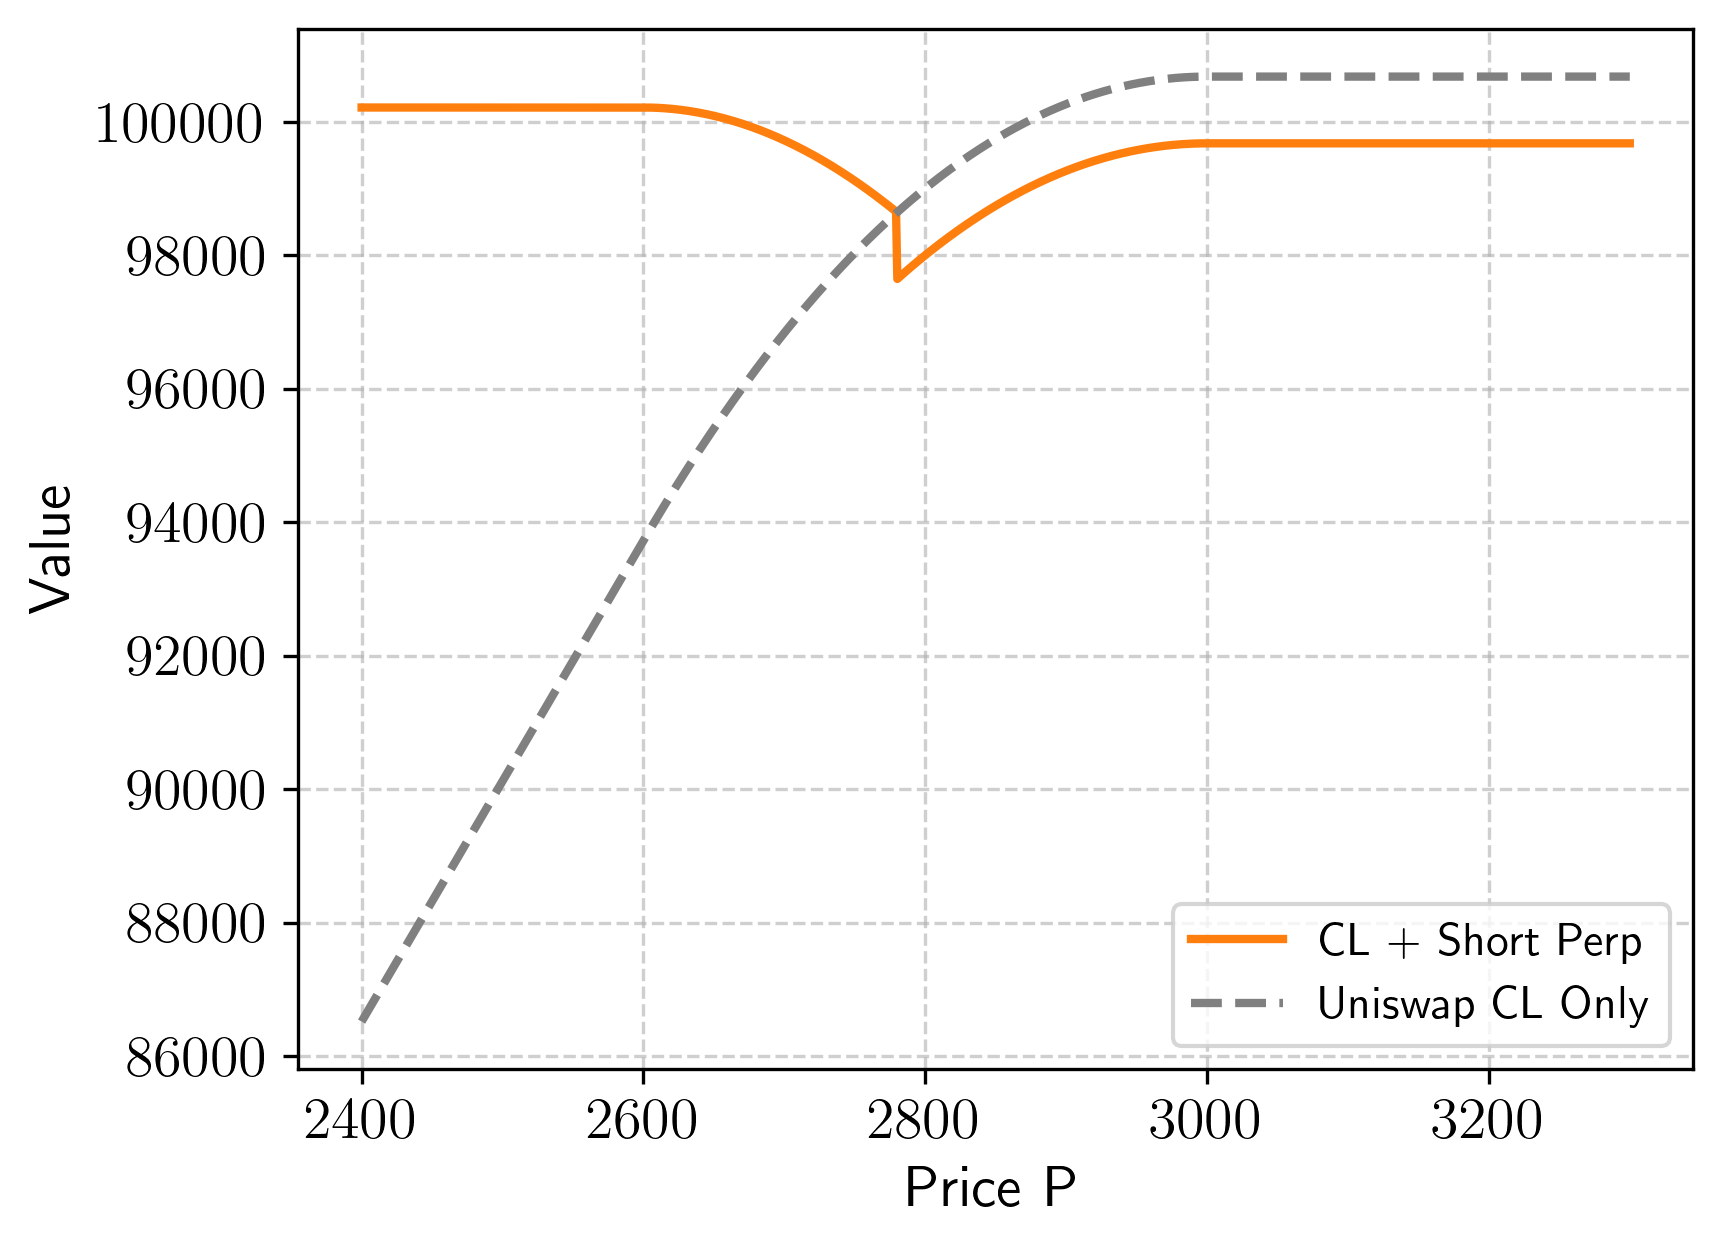
\includegraphics[width=0.9\columnwidth]{img_math/combined_short.png}
\caption{Payoff of an LP position with a short perpetual hedge.}
\label{fig:combined-short}
\justifying

\medskip
In contrast, the Multi Short Perpetual strategy can be applied to pools with two volatile tokens (e.g., BTC and ETH), where the depreciation of one token may result in impermanent loss (IL) denominated in a third currency, such as USDT.

\subsubsection{Long Perpetual Strategy}

\centering
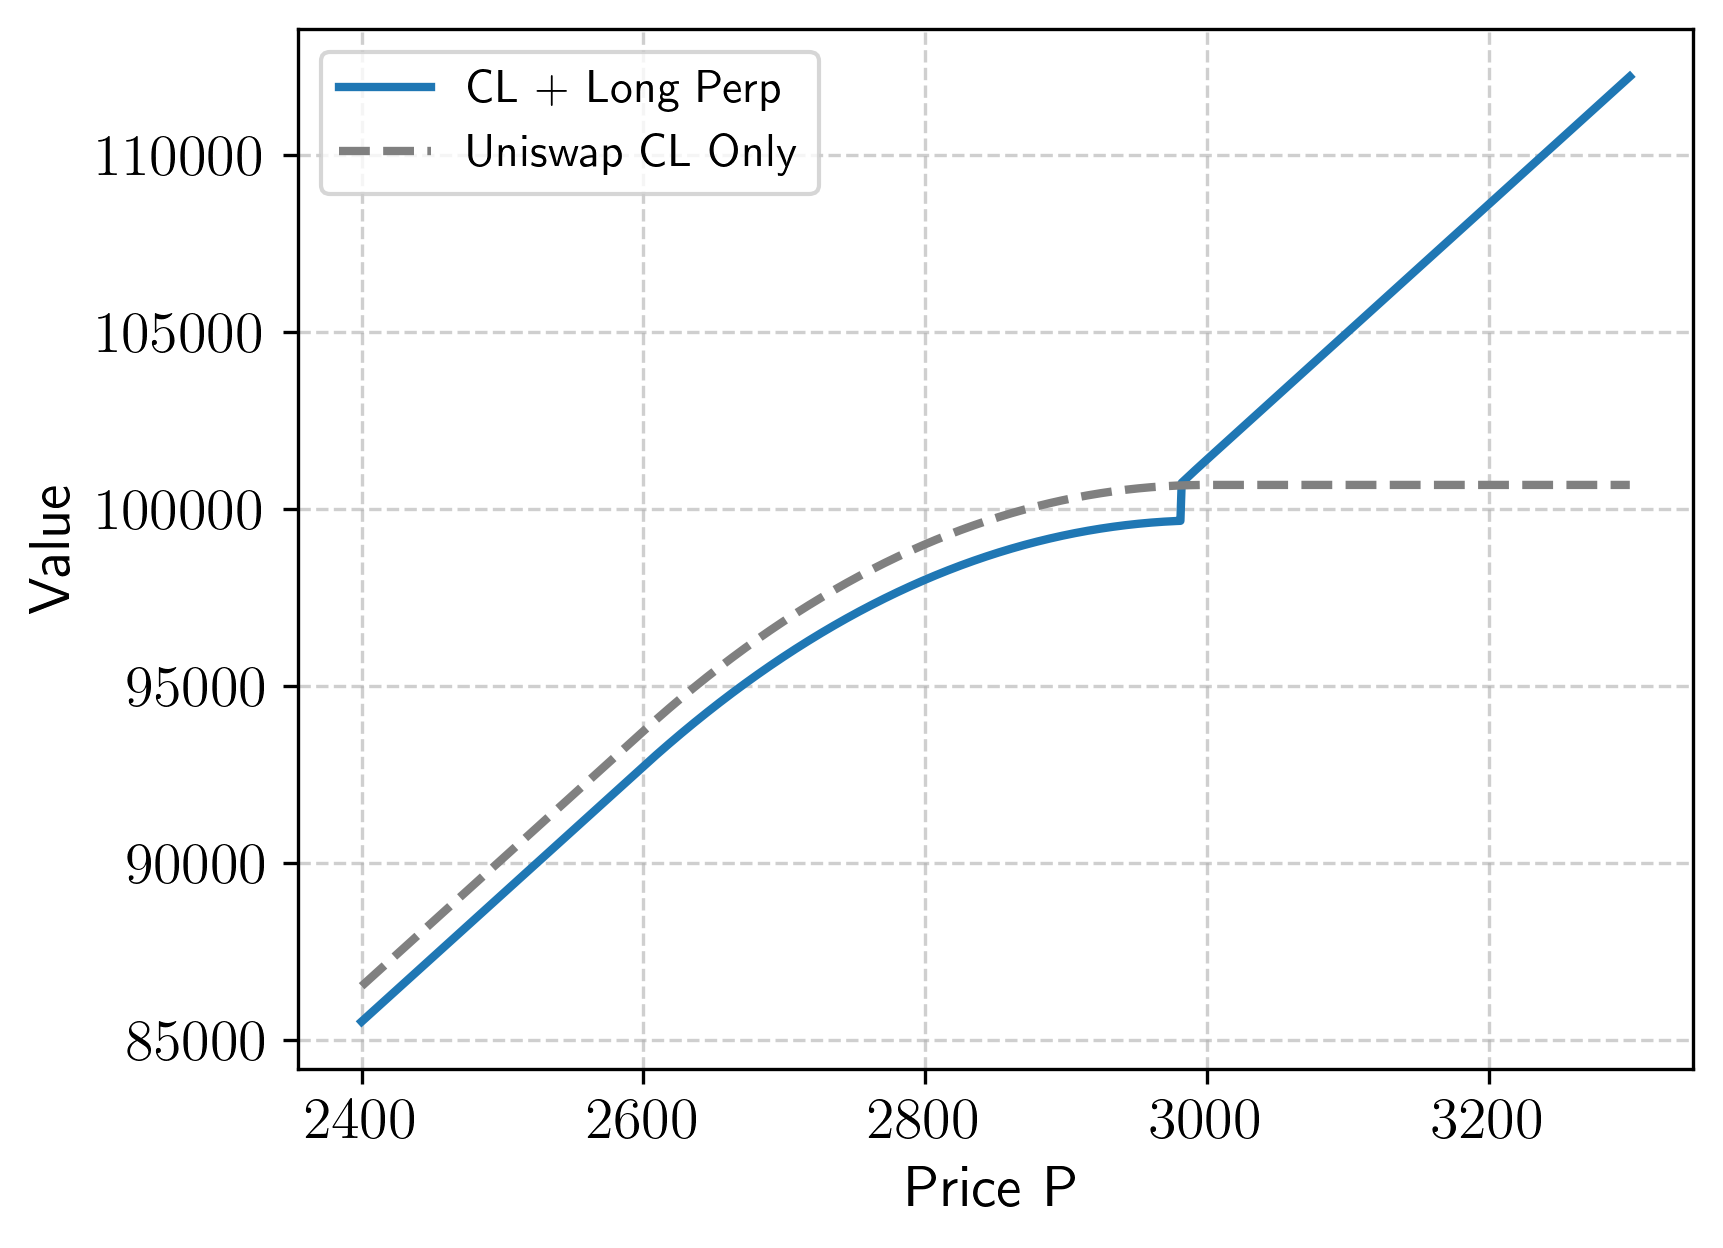
\includegraphics[width=0.9\columnwidth]{img_math/combined_long.png}
\caption{Payoff of an LP position with a long perpetual hedge.}
\label{fig:combined-long}
\justifying

\medskip
Figure~\ref{fig:combined-long} illustrates the combined payoff of a long perpetual hedge with an LP position. This approach is suitable when exposure to the price appreciation of the underlying asset ($token_0$) is desired. Without a hedge, if the price exceeds the upper bound $P_U$, the LP position fully converts to $token_1$, missing out on further upside potential. By incorporating a long perpetual hedge, the strategy captures additional gains from price increases.

\subsubsection{Combined Perpetual Strategy}

\centering
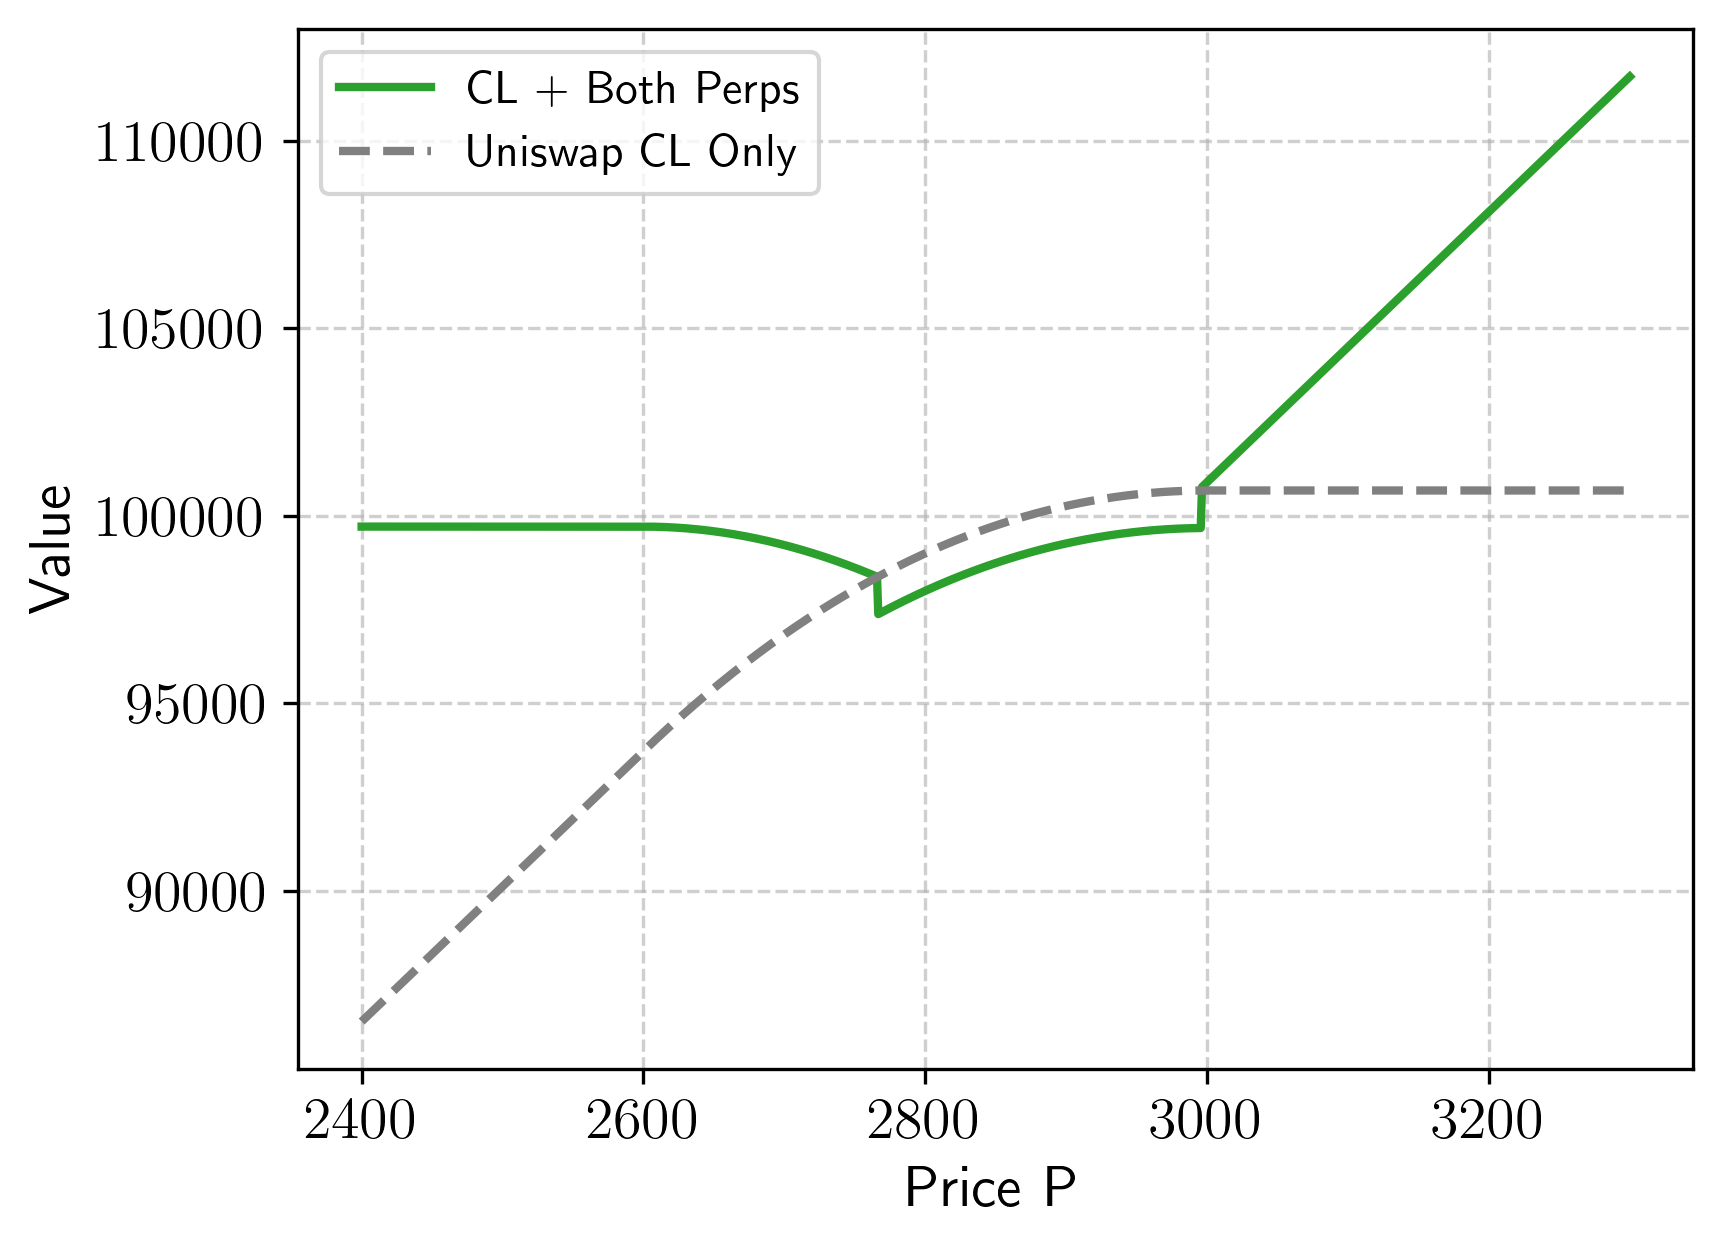
\includegraphics[width=0.9\columnwidth]{img_math/combined_both.png}
\caption{Payoff of an LP position with both short and long perpetual hedges.}
\label{fig:combined-both}
\justifying

\medskip
Figure~\ref{fig:combined-both} illustrates the combined payoff of an LP position hedged with both short and long perpetual positions. This configuration aims to protect against both downside and upside price movements, reducing the risk of the LP position moving out of range. While this combined approach provides significant downside protection and potential upside gains, it requires careful risk management to ensure that liquidation losses do not outweigh the hedging benefits.

\end{multicols}

\end{document}